\documentclass[conference]{IEEEtran}
\IEEEoverridecommandlockouts
% Progress report, prepared 3 November 2026 from repository evidence.
% Diagrams and plot coordinates are in this file; media images are in images/.
% Compile with pdflatex twice (IEEEtran, TikZ and PGFPlots required).
% Compile from docs/: pdflatex main.tex (twice).
% On Overleaf upload main.tex and the images/ directory together.
% No bibliography files, shell escape or simulation are required.
\usepackage{cite}
\usepackage{amsmath,amssymb,amsfonts}
\usepackage{algorithmic}
\usepackage{graphicx}
\graphicspath{{images/}{docs/images/}}
\usepackage{textcomp}
\usepackage{xcolor}
\usepackage{tikz}
\usepackage{pgfplots}
\usetikzlibrary{arrows.meta,positioning,calc}
\pgfplotsset{compat=1.17}
\definecolor{baseblue}{RGB}{205,95,25}
\definecolor{mpcorange}{RGB}{35,93,160}
\pgfplotsset{every axis/.append style={font=\footnotesize,label style={font=\footnotesize},tick label style={font=\scriptsize},legend style={font=\scriptsize,draw=none},grid=major,grid style={gray!20}}}
\tikzset{box/.style={draw,rounded corners=2pt,align=center,font=\footnotesize,minimum height=9mm,inner sep=4pt},arr/.style={-{Latex[length=2mm]},thick}}
\def\BibTeX{{\rm B\kern-.05em{\sc i\kern-.025em b}\kern-.08em T\kern-.1667em\lower.7ex\hbox{E}\kern-.125emX}}
\newcommand{\crossmat}[1]{[#1]_\times}
\newcommand{\sat}{\operatorname{sat}}
\newcommand{\diag}{\operatorname{diag}}
\newcommand{\R}{\mathbb{R}}
\begin{document}
\title{Progress Report on Coupled Predictive Control and Separate Control of an Aerial Manipulator}
\author{\IEEEauthorblockN{Sahil Gajera}
\IEEEauthorblockA{Worcester Polytechnic Institute\\Worcester, MA, USA\\sgajera@wpi.edu}
\and
\IEEEauthorblockN{Aryan Shah}
\IEEEauthorblockA{Worcester Polytechnic Institute\\Worcester, MA, USA\\ajshah1@wpi.edu}}
\maketitle
\begin{abstract}
This progress report compares separate drone and arm control with coupled nonlinear model predictive control for a simulated aerial manipulator. A quadrotor carries a three-joint arm whose own end effector follows a wall trajectory while the drone maintains a fixed hover-position reference. Both controllers operate the same floating-base plant with articulated dynamics, rotor lag, joint actuation limits and native wall contact. The separate baseline exchanges no runtime measurements or commands between its drone and arm controllers. The predictive controller coordinates all seven actuator commands using the coupled model. Under the stated functional criteria the nominal evaluation gives twenty-nine successes in thirty scenarios for predictive control and none for the separate baseline, which nevertheless remains stable and completes its wall trajectories with larger errors. In a wall-free test in which the pad traces a 6 cm radius circle at 2 Hz, the separate baseline loses control in every tested noise seed while predictive control completes the motion, but with almost no rotor-thrust reserve and with computation-deadline overruns. The results establish progress in nominal simulation tracking, with explicit limits on causal attribution, model fidelity and real-time readiness.
\end{abstract}
\begin{IEEEkeywords}
aerial manipulation, nonlinear model predictive control, coupled dynamics, independent control, contact trajectory tracking, simulation
\end{IEEEkeywords}

\section{Introduction}
The implemented task is to maintain a fixed drone base-position reference while a three-degree-of-freedom arm moves its own end effector along a wall in sustained contact. The base remains free to translate and rotate physically; feedback must counter arm reactions and external contact loads. Small changes of attitude are necessary to generate horizontal thrust. Hover does not mean a rigidly fixed or perfectly level base.

Two control architectures are evaluated. Controller B uses independent drone and arm controllers with no runtime exchange of states, commands or task information between them. Controller N uses the coupled drone--arm model to optimize rotor and joint commands together. Both act on the same physically coupled plant. Here, ``decoupled control'' describes B's information structure; it does not mean that arm reactions or wall forces are removed from the physical model.

The comparison evaluates fixed-position hover, end-effector trajectory tracking, contact maintenance, actuator demand and computation time. The primary task uses direct contact at the hand, allows end-effector rotation and maintains contact through a common indentation reference. It does not impose a precision force setpoint or an end-effector orientation target.

The objective is to quantify the benefit of coordinating the drone and arm through a predictive model. Separate feedback control may remain stable while exhibiting larger position errors or repeated contact loss; instability is not required to demonstrate a performance difference.

\subsection{Research Context}
Coupled dynamics are central to aerial manipulation because the underactuated base cannot instantaneously cancel an arbitrary arm-induced wrench. Welde and Kumar formulate the coupled dynamics of a quadrotor with a two-joint arm and establish differential flatness under a specific center-of-mass geometry condition \cite{welde2020}. Welde, Paulos and Kumar subsequently address dynamically feasible end-effector trajectories for underactuated aerial manipulators with an articulated arm \cite{welde2021}. These works motivate joint treatment of vehicle and arm motion; their flatness conditions are not assumed to hold for the assembly used here.

For physical interaction, Alharbat, Gabellieri, Mersha and Franchi incorporate admittance dynamics into an NMPC prediction model \cite{alharbat2025}. Their formulation provides related evidence for predictive interaction control, but the present controller uses position-based contact maintenance on an underactuated quadrotor rather than reproducing their admittance controller. Aerial manipulators in contact have also been controlled with hybrid force/motion schemes and tool-force compensation \cite{malczyk2023}, and fully actuated vehicles have been used for pushing tasks with selective rotational compliance \cite{hui2024}; both differ from the present underactuated, position-based contact task. Adaptive and inverse-dynamics control of a quadrotor with a robotic arm in two layers, an inverse-kinematics layer and a motion-control layer, was proposed in \cite{caccavale2014}; B's arm controller follows that layering in a simplified, non-adaptive form. These publications motivate the modeling and control choices; the B/N performance figures below are results of the present experiments, not results borrowed from the literature.

\section{Assembly, Environment and Assumptions}
\subsection{Physical configuration}
The common plant is simulated in MuJoCo \cite{mujoco} and uses the supplied floating-base assembly adapted to three active joints: yaw $q_1$, shoulder pitch $q_2$ and elbow pitch $q_3$. The wrist is fixed at $\beta=20^\circ$; its hand mass and inertia are retained. A spherical contact button of radius $r_p=12$ mm lies at the hand, between the finger tips. Its center is 64 mm along the local negative hand axis. The compact pad is part of the hand contact geometry. The mount is centered under the airframe, with a continuous visual connection. Figure~\ref{fig:geometry} illustrates the modeled chain rather than a dimensionally exact CAD drawing.

\begin{figure}[t]
\centering
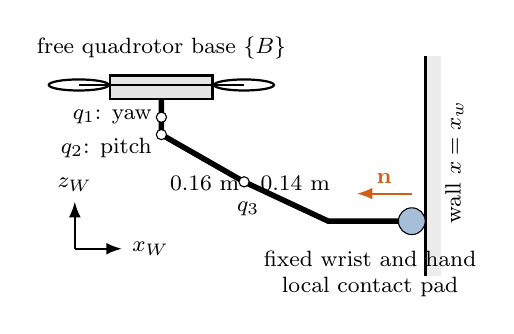
\begin{tikzpicture}[x=1cm,y=1cm,font=\footnotesize]
\fill[gray!15] (3.35,-2.25) rectangle (3.55,.55);
\draw[very thick] (3.35,-2.25)--(3.35,.55);
\node[rotate=90] at (3.72,-.8) {wall $x=x_w$};
\draw[thick,fill=gray!20] (-.65,0) rectangle (.65,.3);
\draw[thick] (-1.05,.18)--(1.05,.18);
\draw[thick] (-1.05,.18) ellipse (.38 and .07);
\draw[thick] (1.05,.18) ellipse (.38 and .07);
\node at (0,.65) {free quadrotor base $\{B\}$};
\draw[line width=2pt] (0,0)--(0,-.45)--(1.05,-1.05)--(2.12,-1.55)--(3.18,-1.55);
\foreach \x/\y in {0/-.23,0/-.45,1.05/-1.05}{\draw[fill=white] (\x,\y) circle (.065);}
\draw[fill=mpcorange!40] (3.18,-1.55) circle (.17);
\node[left] at (0,-.23) {$q_1$: yaw};
\node[left] at (0,-.62) {$q_2$: pitch};
\node[below] at (.55,-.85) {0.16 m};
\node[below] at (1.1,-1.18) {$q_3$};
\node[above] at (1.7,-1.28) {0.14 m};
\node[below,align=center] at (2.65,-1.8) {fixed wrist and hand\\local contact pad};
\draw[arr,baseblue] (3.18,-1.2)--(2.48,-1.2) node[midway,above] {$\mathbf n$};
\draw[arr] (-1.1,-1.9)--(-.5,-1.9) node[right] {$x_W$};
\draw[arr] (-1.1,-1.9)--(-1.1,-1.3) node[above] {$z_W$};
\end{tikzpicture}
\caption{Schematic of the common plant. The drone and arm are physically coupled for both B and N. Wall trajectories lie in the world $y$--$z$ plane; the schematic shows a side projection.}
\label{fig:geometry}
\end{figure}

\begin{table}[t]
\caption{Declared Model and Task Parameters}
\label{tab:parameters}
\centering\footnotesize
\begin{tabular}{p{.46\columnwidth}p{.45\columnwidth}}
\hline
Quantity & Value or status\\\hline
Airframe / arm and hand mass & 1.05 / 0.47 kg\\
Total mass & 1.52 kg\\
Link masses (yaw, upper, forearm, hand) & 0.12, 0.15, 0.10, 0.10 kg\\
Root offset / shoulder offset & 35 / 50 mm downward\\
Upper arm / forearm length & 0.16 / 0.14 m\\
Rotor positions in base $x,y$ & $(\pm0.10,\pm0.10)$ m\\
Rotor thrust range & 0.1--10 N per rotor\\
Maximum rotor speed & 1800 rad/s\\
Reaction-moment/thrust ratio & 0.016 m\\
Motor rise / fall time constant & 0.04 / 0.06 s\\
Joint torque cap / stall torque & 1 / 3 N$\cdot$m\\
Joint no-load speed & 8.06 rad/s\\
Joint viscous damping & 0.01 N$\cdot$m$\cdot$s/rad\\
Contact stiffness / damping & 600 N/m / 8 N$\cdot$s/m\\
Friction coefficient & 0.15\\
Nominal indentation & 1 mm\\
Operational $q_1$ & $[-35,35]^\circ$\\
Operational $q_2$ / $q_3$ & $[-80,-5]^\circ$ / $[-125,-30]^\circ$\\
Physics step / N period & 0.25 / 20 ms\\\hline
\end{tabular}
\end{table}

\subsection{Provenance and physical limits}
Table~\ref{tab:parameters} summarizes the configuration. Body masses and inertias are supplied simulation properties, not parameters identified from a built robot. The rotor coefficients, lag constants, contact law and continuous servo rating include design assumptions. The servo is modeled as an XM430-W210-class actuator, but the assumed 1 N$\cdot$m continuous limit is not a validated thermal rating. Likewise, the airframe XML does not establish measured thrust or motor-response curves.

Mechanical joint ranges are wider than the operational workspace. Operational limits restrict planned motion; the physics engine does not rigidly enforce those narrower ranges. Sampled checks establish feasibility only for the tested nominal paths. They do not certify all link, finger and propeller clearances throughout arbitrary dynamic motion. Near-wall aerodynamic effects and hardware sensing fidelity are not established by these experiments.

\section{Kinematics and Coupled Dynamics}
The following equations distinguish established mechanics from this robot's particular geometry and numerical approximations. Literature citations identify the underlying formulations; the three-joint chain, calibrated constants and controller tuning are specific to this implementation. A matching mathematical structure does not imply that the complete controller or its stability guarantees were reproduced from the cited work.
\subsection{State, frames and end-effector motion}
Let $\mathbf p\in\R^3$ be the base origin in world coordinates, $Q$ a unit quaternion in scalar-first order, and $R(Q)$ the body-to-world rotation. Let $\mathbf v$ be world linear velocity, $\boldsymbol\omega$ body angular velocity, $\mathbf q=[q_1,q_2,q_3]^T$, and $\boldsymbol\Omega\in\R^4$ actual rotor speeds. The stored state and commanded input are
\begin{align}
\mathbf x&=(\mathbf p,Q,\mathbf v,\boldsymbol\omega,\mathbf q,\dot{\mathbf q},\boldsymbol\Omega)\in\R^{23},\label{eq:state}\\
\mathbf u&=(\boldsymbol\Omega_{\rm cmd},\boldsymbol\tau_{\rm cmd})\in\R^7.
\end{align}
The 23 stored components include the redundant quaternion coordinate. The floating base and arm have nine generalized velocity degrees of freedom,
$\boldsymbol\nu=(\mathbf v,\boldsymbol\omega,\dot{\mathbf q})\in\R^9$.

The transform composition and Jacobian construction follow standard rigid-body and serial-chain kinematics \cite[chs.~3--5]{lynch2017}. Applying them to this assembly, with $\mathbf e_z=(0,0,1)^T$, gives the following joint orientations and origins expressed in the base frame:
\begin{align}
R_1&=R_z(q_1),& \mathbf o_1&=(0,0,-0.035)^T,\\
R_2&=R_1R_y(q_2),& \mathbf o_2&=\mathbf o_1-0.05R_1\mathbf e_z,\\
R_3&=R_2R_y(q_3),& \mathbf o_3&=\mathbf o_2-0.16R_2\mathbf e_z,\\
R_h&=R_3R_y(\beta),& \mathbf o_4&=\mathbf o_3-0.14R_3\mathbf e_z.
\end{align}
The corresponding floating-base point-velocity decomposition follows the same kinematic construction as \cite[Sec.~III-B, eqs.~(11)--(16)]{welde2020}, expressed here with world linear velocity and body angular velocity. The pad-center position and velocity are
\begin{align}
\mathbf r_T(\mathbf q)&=\mathbf o_4-0.064R_h\mathbf e_z,\\
\mathbf p_T&=\mathbf p+R\mathbf r_T,\label{eq:fk}\\
\dot{\mathbf p}_T&=\mathbf v-R\crossmat{\mathbf r_T}\boldsymbol\omega
 +RJ_q\dot{\mathbf q}=J_T\boldsymbol\nu,\label{eq:tipvel}
\end{align}
where $J_q=\partial\mathbf r_T/\partial\mathbf q$ and $\crossmat{\mathbf a}\mathbf b=\mathbf a\times\mathbf b$. Equation~\eqref{eq:tipvel} makes the three sources of tip motion explicit: base translation, base rotation and joint motion. Limiting base velocity alone does not bound impact speed.

\subsection{Articulated mass matrix and reaction forces}
For each rigid body $i$, let $J_{v,i}$ and $J_{\omega,i}$ map $\boldsymbol\nu$ into world linear and angular velocities of its center of mass. With world inertia $I_i^W$, the kinetic-energy construction of \cite[Sec.~III-B, eqs.~(17)--(20)]{welde2020} gives the following mass matrix, extended here from that paper's two-joint arm to all bodies in the present three-joint assembly:
\begin{equation}
M=\sum_i\left(m_iJ_{v,i}^TJ_{v,i}+J_{\omega,i}^TI_i^WJ_{\omega,i}\right).
\label{eq:mass}
\end{equation}
The manipulator-equation structure follows \cite[Sec.~III-B, eq.~(8)]{welde2020}. External contact enters through the Jacobian-transpose virtual-work mapping \cite[Sec.~5.2 and ch.~8]{lynch2017}. With this project's rotor actuation and joint damping, the equations implemented independently using CasADi \cite{casadi} are
\begin{equation}
M\dot{\boldsymbol\nu}+\mathbf b+\mathbf g
=\mathbf w_r+S^T(\boldsymbol\tau-D\dot{\mathbf q})+J_C^T\mathbf f_C,
\label{eq:dynamics}
\end{equation}
where $S=[0_{3\times6}\ I_3]$, $\mathbf b$ contains velocity-dependent inertial terms, $\mathbf g$ is generalized gravity, and $\mathbf w_r$ is the rotor generalized force. The predictor obtains the bias from directional derivatives of body Jacobians and gyroscopic terms; it does not read MuJoCo's runtime mass matrix or bias.

Partitioning \eqref{eq:dynamics} into base and arm coordinates gives the following algebraic rearrangement; it is not an additional approximation or a separately fitted coupling model:
\begin{equation}
\begin{bmatrix}M_{bb}&M_{ba}\\M_{ab}&M_{aa}\end{bmatrix}
\begin{bmatrix}\dot{\boldsymbol\nu}_b\\\ddot{\mathbf q}\end{bmatrix}
+\begin{bmatrix}\mathbf h_b\\\mathbf h_a\end{bmatrix}
=\begin{bmatrix}\mathbf w_b\\\boldsymbol\tau\end{bmatrix}
+J_C^T\mathbf f_C,
\label{eq:blocks}
\end{equation}
with damping absorbed into $\mathbf h$ here. In particular, $-M_{ba}\ddot{\mathbf q}$ contributes to base acceleration. Changing arm posture also changes mass distribution and gravity/rotor moment balance. These effects remain in the plant for B; separation applies to its control interfaces, not to the simulated mechanics.

Summing the Newton--Euler balances over the assembly cancels internal wrenches \cite[Secs.~8.2--8.3]{lynch2017}. For the external loads represented here, the resulting whole-system momentum diagnostic is
\begin{align}
m\ddot{\mathbf c}&=R\mathbf e_z\sum_i f_i-mg\mathbf e_z+\mathbf f_C,\label{eq:linearbalance}\\
\dot{\mathbf H}_{c}&=\sum_i(\mathbf p_i-\mathbf c)\times R\mathbf e_z f_i
+R\mathbf m_{\rm yaw}+(\mathbf p_C-\mathbf c)\times\mathbf f_C.
\label{eq:angularbalance}
\end{align}
Here $\mathbf c$ is the total center of mass and $\mathbf H_c$ its angular momentum in world coordinates. Internal joint torques cancel from these whole-system balances. Consequently, base displacement and center-of-mass displacement are different measurements. A stationary base can coexist with a moving system center of mass while the arm moves.

\subsection{Propulsion and joint actuation}
Rotor wrench allocation follows the moment-arm and alternating reaction-torque construction in \cite[Sec.~II]{lee2011}, with signs converted to the positive-body-$z$ thrust convention used here. We assume a quadratic static thrust map and first-order speed lag; their coefficients are simulation choices rather than parameters taken from that reference. The resulting rotor model is
\begin{align}
f_i&=k_f\Omega_i^2, &k_f&=10/1800^2,\\
\begin{bmatrix}T\\M_x\\M_y\\M_z\end{bmatrix}
&=A\mathbf f,&A_{:,i}&=(1,y_i,-x_i,s_i\kappa)^T,\label{eq:allocation}\\
\dot\Omega_i&=(\Omega_{{\rm cmd},i}-\Omega_i)/\tau_i,
\end{align}
where $s_i\in\{+1,-1,+1,-1\}$ and $\kappa=0.016$ m. The plant integrates the lag exactly over each physics step, choosing the rise or fall constant according to command direction. The predictor smooths that switch. Rotor commands are limited to $[180,1800]$ rad/s, equivalent to the stated static thrust limits.

The driving-torque envelope is an assumed linear interpolation between the declared stall torque and no-load speed, clipped by the assumed continuous-torque cap. It is not a fitted servo curve or a formula taken from an aerial-manipulation paper. The plant uses
\begin{equation}
\tau_{\max}(\dot q)=\max\!\left(0,\min\!\left(\tau_c,\tau_s\left(1-\frac{|\dot q|}{\omega_{\rm nl}}\right)\right)\right),
\label{eq:envelope}
\end{equation}
with braking allowed up to $\tau_c=1$ N$\cdot$m. Importantly, the current N predictor applies a constant torque bound rather than this speed-dependent envelope. Agreement at low joint speed therefore does not establish actuator fidelity at the circle-test boundary.

\subsection{Wall contact and material-point velocity}
The outward wall normal is $\mathbf n=(-1,0,0)^T$. With wall coordinate $x_w=0.8$ m, the gap and positive closing speed are
\begin{equation}
g_c=x_w-p_{T,x}-r_p,\qquad v_c=-\dot g_c=-\mathbf n^T J_T\boldsymbol\nu.
\end{equation}
Using the rigid-body point-velocity relation \cite[ch.~3]{lynch2017}, the material point on the sphere facing the wall is $\mathbf p_C=\mathbf p_T-r_p\mathbf n$. Its velocity, including rotation, is
\begin{equation}
\mathbf v_C=J_C\boldsymbol\nu,\qquad J_C=J_T+r_p\crossmat{\mathbf n}J_{\omega,T}.
\end{equation}
The normal law is this implementation's smoothed unilateral spring--damper approximation. Its softplus penetration, logistic activation and piecewise force smoothing are numerical design choices, not equations attributed to the predictive-admittance paper. Tangential force regularizes the Coulomb sliding law \cite[Sec.~12.2.1]{lynch2017}. Writing $\delta_\epsilon=\epsilon_g\log(1+e^{-g_c/\epsilon_g})$ and $\chi_\epsilon=(1+e^{g_c/\epsilon_g})^{-1}$, the predictor uses
\begin{align}
a&=k\delta_\epsilon+c v_c,\\
F_n&=\chi_\epsilon\psi(a),\label{eq:contact}\\
\psi(a)&=\begin{cases}0,&a\leq0,\\a^2/(2\epsilon_F),&0<a<\epsilon_F,\\a-\epsilon_F/2,&a\geq\epsilon_F,\end{cases}\\
\mathbf f_t&=-\mu F_n\frac{\mathbf v_t}{\sqrt{\mathbf v_t^T\mathbf v_t+v_\epsilon^2}},\quad
\mathbf v_t=(I-\mathbf n\mathbf n^T)\mathbf v_C,\\
\mathbf f_C&=\mathbf nF_n+\mathbf f_t.
\end{align}
Defaults are $\epsilon_g=10^{-5}$ m, $\epsilon_F=10^{-3}$ N and $v_\epsilon=2\times10^{-3}$ m/s. These smooth equations are the prediction approximation; MuJoCo uses native compliant contact with a calibrated stiffness scale of 0.95. Equality of instantaneous rigid-body dynamics does not imply equality of impact peaks or friction transitions.

Setting acceleration to zero in \eqref{eq:linearbalance} gives the following force-balance consequence, under approximate steady contact without significant vertical friction:
\begin{equation}
T\cos\theta\simeq mg,\qquad T\sin\theta\simeq F_n,
\quad \theta\simeq\tan^{-1}(F_n/mg).
\label{eq:tilt}
\end{equation}
Tilt supplies horizontal force; differential rotor thrust supplies the balancing moment. Wall contact need not cause visible wobble if those loads are compensated.

\section{Common Task and Reference Generation}
\subsection{Contact trajectory}
The task commands the pad center, with a normal indentation $\delta_r=1$ mm and a planar trajectory $(y_r(s),z_r(s))$:
\begin{equation}
\mathbf p_{T,r}(s)=(x_w-r_p+\delta_r,\ y_r(s),\ z_r(s))^T.
\end{equation}
The drone base reference remains fixed at $(0.508,0,1.2)$ m. The nominal wall patch is centered at $(y,z)=(0,1.04)$ m. Examples are an 80 mm horizontal line, a circle of radius 25 mm and an open polyline with a rounded corner. The polyline is open, with a rounded change of direction.

Reference timing uses the standard fifth-order rest-to-rest polynomial with zero endpoint velocity and acceleration \cite[Secs.~9.1--9.2]{lynch2017}. The velocity and acceleration below then follow by the chain rule:
\begin{align}
s(\xi)&=10\xi^3-15\xi^4+6\xi^5,\quad 0\leq\xi\leq1,\\
\dot{\mathbf p}_{T,r}&=\mathbf p'_{T,r}(s)\dot s,\\
\ddot{\mathbf p}_{T,r}&=\mathbf p''_{T,r}(s)\dot s^2+\mathbf p'_{T,r}(s)\ddot s.
\end{align}
During progress ramps and recovery, velocity is scaled by the actual progress rate so that position and velocity references remain consistent. A finite-difference check gives a maximum discrepancy of $1.2\times10^{-6}$ m/s.

\begin{figure}[t]
\centering
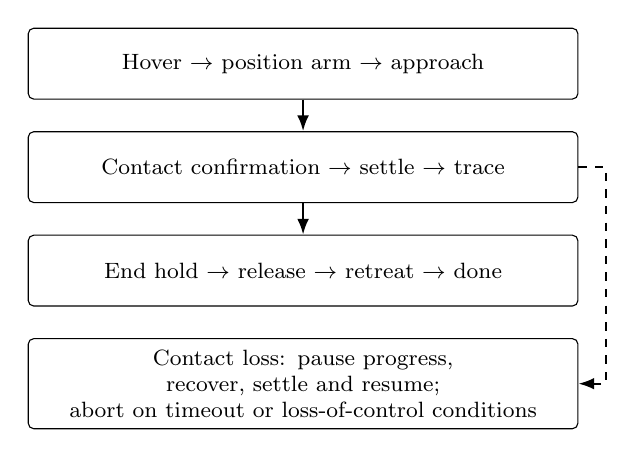
\begin{tikzpicture}[node distance=4mm]
\node[box,text width=6.7cm] (a) {Hover $\rightarrow$ position arm $\rightarrow$ approach};
\node[box,text width=6.7cm,below=of a] (b) {Contact confirmation $\rightarrow$ settle $\rightarrow$ trace};
\node[box,text width=6.7cm,below=of b] (c) {End hold $\rightarrow$ release $\rightarrow$ retreat $\rightarrow$ done};
\draw[arr] (a)--(b);\draw[arr] (b)--(c);
\node[box,text width=6.7cm,below=of c] (d) {Contact loss: pause progress, recover, settle and resume;\\abort on timeout or loss-of-control conditions};
\draw[arr,dashed] (b.east)--++(.35,0)|-(d.east);
\end{tikzpicture}
\caption{Task flow shared in purpose by B and N. B's task uses its own gap reference rather than drone-derived pad position; arm-side contact-force sensing is retained.}
\label{fig:task}
\end{figure}

\subsection{Contact persistence and equal task intent}
Contact confirmation requires force above 0.15 N for 0.06 s; loss detection uses 0.08 N and 0.10 s. These durations are in seconds rather than control samples, avoiding a fourfold detection-rate difference between B and N. Contact loss pauses progression and invokes recovery. Figure~\ref{fig:task} summarizes the sequence.

Both controllers receive the same intended indentation and tangential path. The nominal elastic preload is $k\delta_r\simeq0.6$ N, but there is no exact force-tracking objective. Different measured forces are therefore outcomes of task execution. Equal force histories are not imposed. In particular, weak or intermittent contact can reduce B's tilt while also reducing its task success. Smaller tilt alone is not evidence of better control.

\section{Controllers B and N}
\subsection{B: separate drone and arm controllers}
Figure~\ref{fig:architecture} shows the runtime information boundaries. B's drone controller receives base position, attitude, linear and angular velocity, and rotor speeds. It uses fixed total mass, nominal locked-posture center of mass and inertia, plus a hover trim initialized once from rotor telemetry. It receives no arm state, trajectory, task phase or contact force. These fixed calibration constants are disclosed; B is not a mass-ignorant bare-drone controller.

B's drone loop combines PID position feedback with the geometric attitude-error construction of \cite[Secs.~IV--V]{lee2011}. Its integral terms, fixed-inertia scaling, trim and latency extrapolation are implementation adaptations, so the source's stability result is not claimed for B. Using position error $\mathbf e_p=\hat{\mathbf p}-\mathbf p_r$, its outer loop is
\begin{align}
\mathbf a_d&=-K_p\mathbf e_p-K_v\mathbf v-K_i\mathbf i_p,\\
\mathbf i_p^+&=\sat(\mathbf i_p+\mathbf e_p\Delta t),\\
\mathbf F_d&=m(\mathbf a_d+g\mathbf e_z).
\end{align}
The desired attitude aligns body thrust with $\mathbf F_d$ at fixed nominal yaw. With $\mathbf e_R=\tfrac12(R_d^TR-R^TR_d)^\vee$, the moment command is
\begin{align}
\mathbf M_d={}&-J_0(\omega_a^2\mathbf e_R+2\zeta\omega_a\boldsymbol\omega
+K_{iR}\mathbf i_R)\nonumber\\
&+\boldsymbol\omega\times J_0\boldsymbol\omega
+\mathbf r_{c,0}\times(T\mathbf e_z)+\mathbf M_{\rm trim}.
\end{align}
Allocation uses \eqref{eq:allocation}, followed by per-rotor clipping. The measured state is extrapolated over $1.5\Delta t$ for latency compensation. B uses $K_p=4.7908$, $K_v=5.1545$, $K_i=1.2254$, $\omega_a=11.5777$, $\zeta=1$, and $K_{iR}=454.269$ in the implementation's SI convention. Its optional motor-lag inversion gain is zero.

The arm controller sees only joint position and velocity and its own task reference. It solves inverse kinematics under an assumed fixed base pose; during contact it assumes pitch $\tan^{-1}(F_r/mg)$ using its own intended preload $F_r=k\max(-g_r,0)$. It does not use measured base pose. Its torque law combines reference-model inverse-dynamics feedforward and joint PD feedback, following the two-layer structure (inverse kinematics, then model-based joint control) of \cite{caccavale2014} and the model-based control principles in \cite[Sec.~11.4]{lynch2017}. Unlike full computed-torque feedback linearization, the dynamic terms here are evaluated at the reference and the PD terms are added directly as torques. The arm's nominal contact-load compensation uses the virtual-work mapping of \cite[Sec.~5.2]{lynch2017}:
\begin{align}
\boldsymbol\tau_B={}&M_{aa,r}\ddot{\mathbf q}_r+\mathbf b_{a,r}+\mathbf g_{a,r}
+D\dot{\mathbf q}_r-J_{C,a,r}^T\mathbf f_r\nonumber\\
&+K_{pq}(\mathbf q_r-\mathbf q)+K_{dq}(\dot{\mathbf q}_r-\dot{\mathbf q}),
\label{eq:baselinearm}
\end{align}
with $K_{pq}=0.9952$, $K_{dq}=0.0185$ and clipping at $\pm1$ N$\cdot$m. Reference joint derivatives are obtained from the arm Jacobian. Thus B's arm has joint feedback and arm-model feedforward: it is not an open-loop torque replay. What it lacks is feedback of actual world pad position and changing base motion. Newton inverse kinematics is not yet comprehensively guarded against unreachable targets or singularities.

B operates at 200 Hz with one 5 ms command period of latency. Recorded separation checks perturb arm information without changing drone outputs and vice versa over 300 steps. Separate control does not remove physical reaction forces, nor does it guarantee instability.

\begin{figure*}[t]
\centering
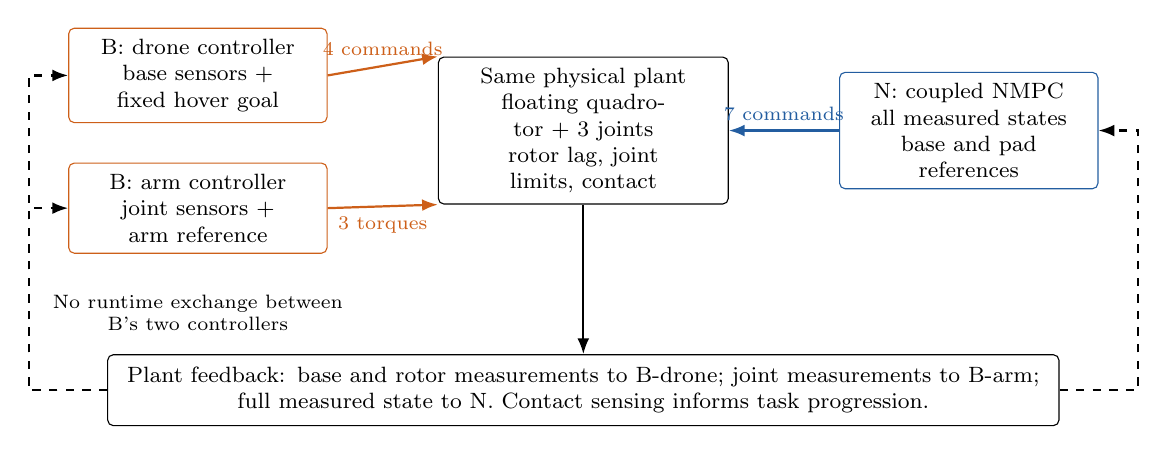
\begin{tikzpicture}[node distance=5mm]
\node[box,text width=3.0cm,draw=baseblue] (bd) {B: drone controller\\base sensors + fixed hover goal};
\node[box,text width=3.0cm,draw=baseblue,below=of bd] (ba) {B: arm controller\\joint sensors + arm reference};
\node[box,text width=3.4cm,right=14mm of bd,yshift=-7mm] (plant) {Same physical plant\\floating quadrotor + 3 joints\\rotor lag, joint limits, contact};
\node[box,text width=3.0cm,draw=mpcorange,right=14mm of plant] (nn) {N: coupled NMPC\\all measured states\\base and pad references};
\draw[arr,baseblue] (bd.east)--node[above,font=\scriptsize] {4 commands}(plant.north west);
\draw[arr,baseblue] (ba.east)--node[below,font=\scriptsize] {3 torques}(plant.south west);
\draw[arr,mpcorange] (nn.west)--node[above,font=\scriptsize] {7 commands}(plant.east);
\node[font=\scriptsize,align=center,below=4mm of ba] {No runtime exchange between\\B's two controllers};
\node[box,text width=11.8cm,below=19mm of plant] (sense) {Plant feedback: base and rotor measurements to B-drone; joint measurements to B-arm;\\full measured state to N. Contact sensing informs task progression.};
\draw[arr] (plant.south)--(sense.north);
\draw[arr,dashed] (sense.west)-|([xshift=-5mm]bd.west)--(bd.west);
\draw[arr,dashed] (sense.west)-|([xshift=-5mm]ba.west)--(ba.west);
\draw[arr,dashed] (sense.east)-|([xshift=5mm]nn.east)--(nn.east);
\end{tikzpicture}
\caption{Comparison architecture. B and N are evaluated in separate runs on the same plant model. The diagram does not imply that their commands are applied simultaneously. B's drone and arm exchange no runtime information, whereas N optimizes their actuation jointly.}
\label{fig:architecture}
\end{figure*}

\subsection{N: coupled nonlinear predictive control}
N uses a ten-stage horizon at $h=20$ ms, giving 0.2 s preview. The prediction map $\Phi_h$ applies RK4 with four substeps of 5 ms and renormalizes the quaternion at the end of each control interval. Before optimization, the measured state is propagated with the pending command for one period to account for actuation latency.

The discretized optimal-control structure, nonlinear least-squares objective and softened inequalities follow the class of NMPC formulations supported by acados \cite{acados}. The particular residuals, bounds, horizon and slack penalties below are this project's design choices; they are not a copied objective from the aerial-interaction papers. The multiple-shooting problem is
\begin{align}
\min_{X,U,S}\quad &\sum_{j=0}^{H-1}\|\mathbf r_j\|_2^2+\|\mathbf r_H\|_2^2
+\rho\sum_{j=0}^{H}(\|\mathbf s_j\|_2^2+\mathbf1^T\mathbf s_j),\label{eq:ocp}\\
\text{subject to}\quad &\mathbf x_0=\hat{\mathbf x}_{\rm apply},\quad
\mathbf x_{j+1}=\Phi_h(\mathbf x_j,\mathbf u_j),\nonumber\\
&\mathbf u_{\min}\leq\mathbf u_j\leq\mathbf u_{\max},\quad
\mathbf h(\mathbf x_j)\leq\mathbf s_j,\quad\mathbf s_j\geq0.\nonumber
\end{align}
Here $H=10$ and $\rho=10^3$. The residual concatenates normalized pad position and velocity error, base position and velocity error, attitude error from level, body angular velocity, joint rates and input increments. The attitude term is weak regularization, not an end-effector pointing objective or a hard level-flight constraint. There is no normal-force error term.

For group $g$, $\mathbf r_g=\sqrt{w_g}\,\mathbf e_g/\boldsymbol\sigma_g$. Position scales are $(1,2,2)$ mm for the pad and 5 mm for the base; velocity scales are 5 mm/s for the pad and 20 mm/s for the base. Angular scales are 0.05 rad for attitude, 0.2 rad/s for body rate and 0.5 rad/s for joint rate. Input increment scales are 100 rad/s for rotor commands and 0.2 N$\cdot$m for torques. The implementation stores square-root weights, not cost coefficients:
\begin{align}
\sqrt{\mathbf w}_{\rm general}&=(2,1,6,2,0.3,1,0.2,0.3),\\
\sqrt{\mathbf w}_{\rm trace}&=(3,1.5,6,2,0.3,1,0.2,0.3).
\end{align}
The order is pad position, pad velocity, base position, base velocity, attitude, body rate, joint rate and input increment.

The 17 soft inequalities cover tilt, both sides of each operational joint range, both signs of joint rate, predicted normal force, closing speed and two point-height clearance approximations. Tilt is limited to $15^\circ$ and joint rate to 3 rad/s through slacks. Rotor command and torque bounds are hard. Soft constraints can be violated and do not replace independent trajectory evaluation. The two point-height constraints do not constitute full collision avoidance.

Production optimization uses acados \cite{acados} with SQP-RTI, Gauss--Newton Hessian approximation and HPIPM with partial condensing. A previous-input augmentation gives a 30-component optimization state. The IPOPT reference shares expressions, but comprehensive numerical solver parity at acquired contact and with active slacks remains open. The implementation shifts the warm start, retries failed solves and can hold the pending command as fallback; absence of fallback alone does not prove constraint satisfaction.

\section{Verification and Experimental Method}
\subsection{Model and stationary-hover verification}
Recorded checks compare independently formed kinematics, the full $9\times9$ mass matrix, bias and instantaneous accelerations with MuJoCo to approximately $10^{-10}$. Momentum-based physics checks use MuJoCo directly rather than the predictor. Reported sliding-contact linear-balance residuals include $1.7\times10^{-6}$ N for B and $5.7\times10^{-5}$ N for N. A known 0.3 N external-force check reproduces center-of-mass acceleration within 0.05\%.

Joint-pulse and fixed-command diagnostics support transmission of internal arm reactions to the base. B maintains stationary hover at four tested postures with sensor noise and recovers from velocity kicks. These checks establish a stable hover baseline for the comparison, while leaving the response to moving-arm trajectories to the experiments below. Instantaneous dynamics agreement does not establish accuracy of discretized impact peaks or full collision avoidance.

\subsection{Metrics and functional acceptance}
The evaluation metrics below are defined for this experiment; their thresholds are task criteria rather than literature-derived guarantees. For samples $k$ over a declared evaluation window $\mathcal W$, the main errors are
\begin{align}
e_{B,\max}&=\max_{k\in\mathcal W}\|\mathbf p_k-\mathbf p_r\|,\\
e_{T,\rm rms}&=\sqrt{\frac{1}{|\mathcal W|}\sum_{k\in\mathcal W}\|\mathbf p_{T,k}-\mathbf p_{T,r,k}\|^2},\\
\theta_k&=\cos^{-1}\!\left(\operatorname{clip}(\mathbf e_z^TR_k\mathbf e_z,-1,1)\right),\\
r_{\rm down}&=\min_{i,t}f_i(t)-f_{\min},\quad
r_{\rm up}=f_{\max}-\max_{i,t}f_i(t).
\end{align}
Force peaks and rotor reserves should use physics-resolution samples. Contact validity is scored over contact-intended time, including recovery, rather than only successful trace segments. Whole-run and motion-only RMS values must be distinguished; they are not interchangeable.

\begin{table}[t]
\caption{Functional Criteria Used in the Nominal Gate}
\label{tab:criteria}
\centering\footnotesize
\begin{tabular}{lc}\hline
Metric & Threshold\\\hline
Maximum base-position error & 20 mm\\
Maximum tilt & $15^\circ$\\
Pad tracking RMS & 3 mm\\
Path coverage within 5 mm & $\geq0.95$\\
Endpoint error & $\leq5$ mm\\
Contact-valid fraction & $\geq0.95$\\
Contact losses & $\leq2$\\
Peak normal force & $\leq4$ N\\
Upward and downward rotor reserve & $\geq0.3$ N each\\
Measured gap after retreat & $\geq50$ mm\\\hline
\end{tabular}
\end{table}
Successful completion, absence of unintended contacts and the applicable task criteria are required in addition to individual error values. Free-arm cases require pad tracking even without a contact phase. The gate requires 29 successes from 30 scenarios. Timing is reported separately and is not included in that functional count.

\subsection{Matching and interpretation}
Both runs use the same physical plant, intended task and scenario conditions. Noise is indexed by seed and physical time, giving identical noise samples at coincident sample times. However, B uses 200 Hz with 5 ms latency, while N uses 50 Hz with 20 ms latency and a longer predictive horizon. Controller architecture, information, preview and tuning procedures also differ. Consequently this is a practical comparison, not an isolated test of one inertial cross term or of MPC versus PD at identical bandwidth.

B's measured contact force is lower because the achieved indentation differs. This does not invalidate a same-task comparison: maintaining contact is part of the task. It does prevent claiming that both controllers experienced equal external forces or that their different tilt traces alone measure disturbance-rejection ability. Force, trajectory tracking and base motion must be read together.

\section{Recorded Results}
\subsection{Nominal gate and representative wall trajectories}
The 30-case evaluation contains 27 wall tasks and three free-arm tasks. N completes all 30 and satisfies the functional criteria on 29. Its unsuccessful free-arm case has an initial posture at the $q_2$ operational limit and a reference identified as unreachable within those limits. This case is included as a failure in the reported success count.

B satisfies the combined functional criteria in 0 of 30 scenarios. Its median maximum base error is 29.8 mm and median wall-trace RMS error is 18.3 mm, compared with 0.58 mm and 0.42 mm for N. Table~\ref{tab:gate} summarizes the comparison.

\begin{table}[t]
\caption{B versus N: Nominal Evaluation}
\label{tab:gate}
\centering\footnotesize
\begin{tabular}{lcc}\hline
Quantity & B & N\\\hline
Functional successes / 30 & 0 & 29\\
Median maximum base error (mm) & 29.8 & 0.58\\
Median wall-trace RMS (mm) & 18.3 & 0.42\\\hline
\end{tabular}
\vspace{2pt}
\parbox{.96\columnwidth}{\scriptsize N's worst base error is 113.8 mm on the failed free-arm case. Medians do not describe every scenario.}
\end{table}

Three representative B/N recordings show line, circle and rounded-polyline tracking (Fig.~\ref{fig:wallresults}). B loses contact 11, 9 and 9 times, respectively, with valid fractions approximately 0.78, 0.87 and 0.87. N has no recorded losses and valid fraction 1.00 in these examples. B's trace RMS errors are 17.7, 14.9 and 13.0 mm; N's are 0.345, 0.426 and 0.411 mm. These are three demonstrations, not the complete gate distribution.

\begin{figure}[t]
\centering
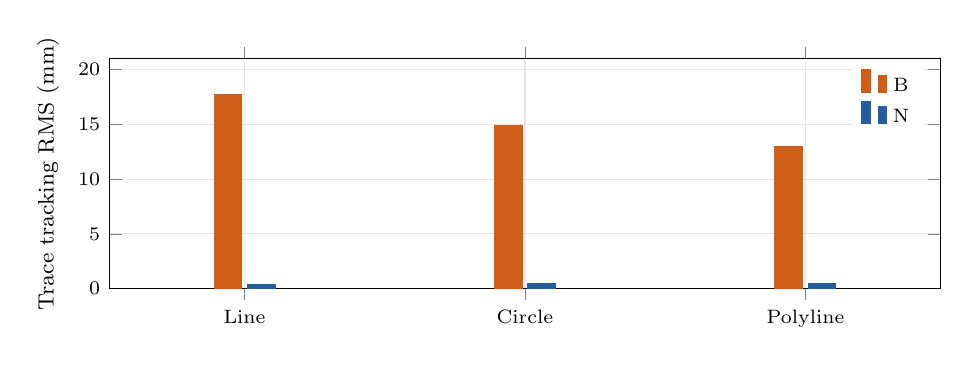
\begin{tikzpicture}
\begin{axis}[width=\columnwidth,height=4.5cm,ybar,bar width=10pt,ymin=0,ymax=21,
 symbolic x coords={Line,Circle,Polyline},xtick=data,ylabel={Trace tracking RMS (mm)},
 legend style={at={(.98,.98)},anchor=north east},enlarge x limits=.24]
\addplot[fill=baseblue,draw=baseblue] coordinates {(Line,17.7) (Circle,14.9) (Polyline,13.0)};
\addplot[fill=mpcorange,draw=mpcorange] coordinates {(Line,.345) (Circle,.426) (Polyline,.411)};
\legend{B,N}
\end{axis}
\end{tikzpicture}
\caption{Recorded wall-trace RMS errors from the three strictly separated B/N demonstrations. Identical reference intent does not imply identical achieved force: B repeatedly loses contact. Values are from the recorded B/N experiments.}
\label{fig:wallresults}
\end{figure}

The actual robot and contact traces are shown in Figs.~\ref{fig:mediawalls} and~\ref{fig:mediapolyline}, extracted from the separated-controller recordings. These are synchronized simulation-time snapshots, not matched task-progress snapshots: B's recovery can delay its progress. Figure~\ref{fig:mediatimeseries} reproduces the recorded line-run time series, showing how contact loss, base drift and tangential error evolve together.

\begin{figure*}[p]
\centering
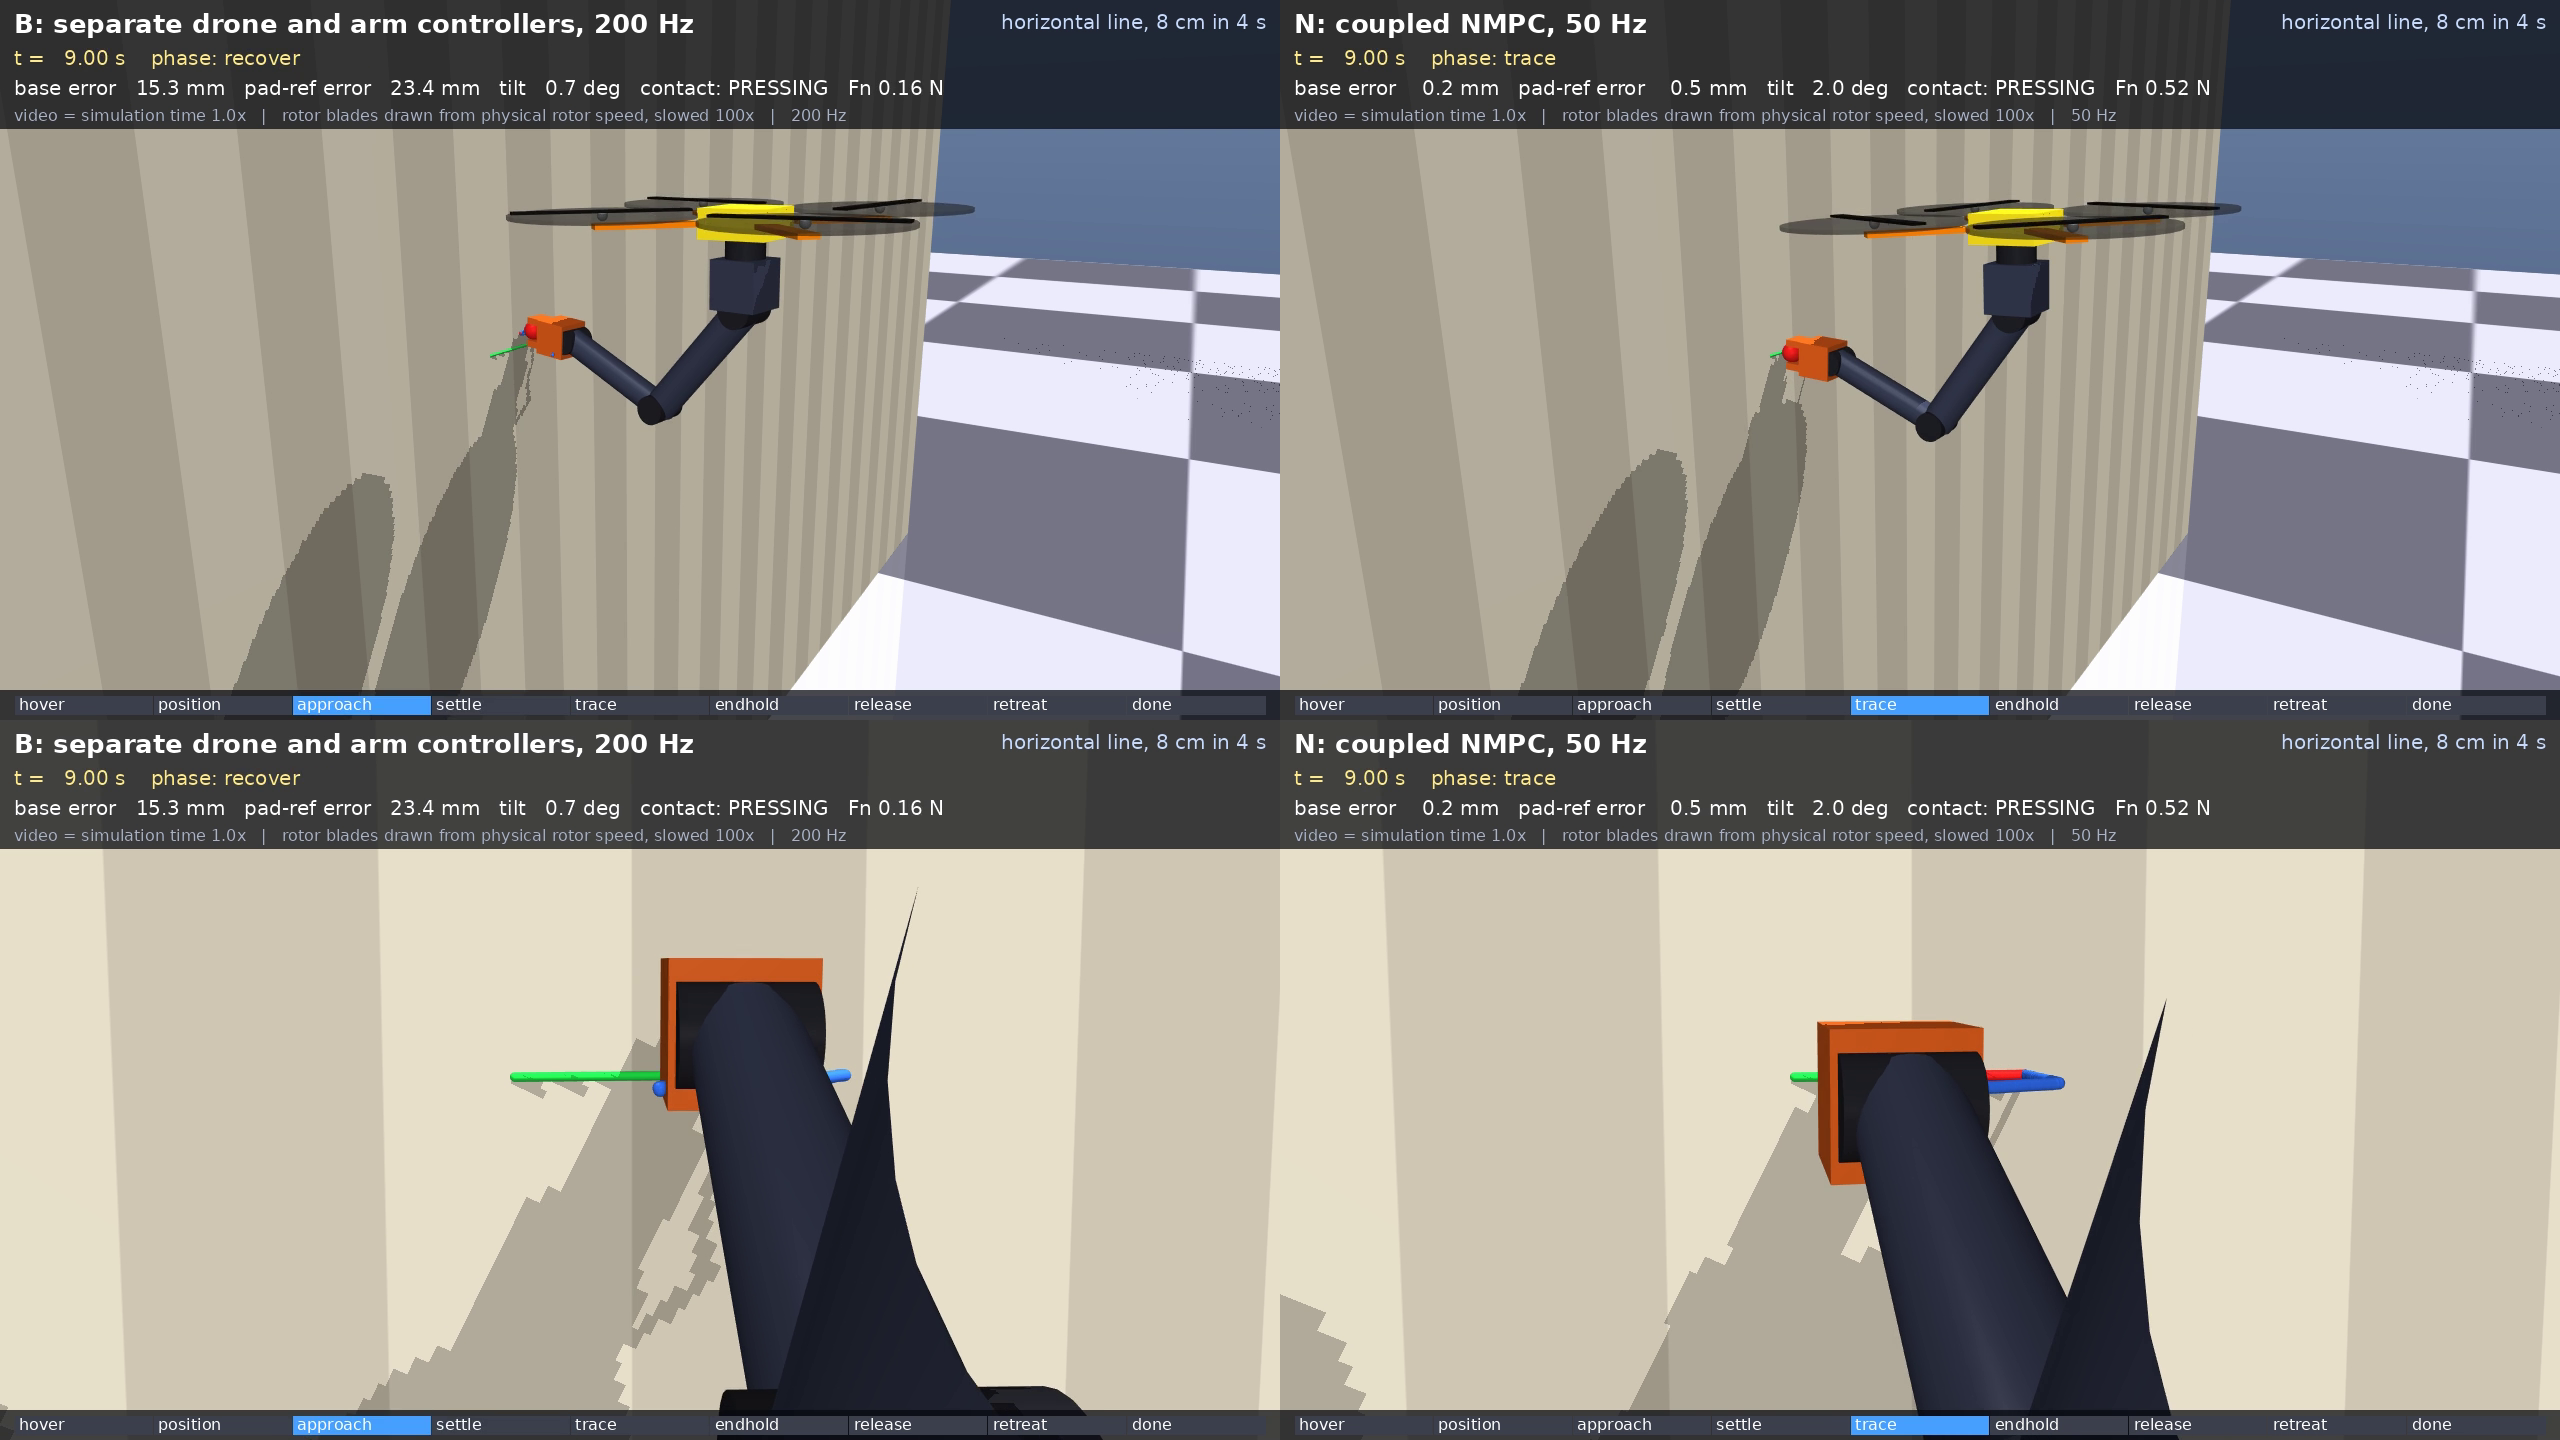
\includegraphics[width=\textwidth]{bn_line_frame.png}\\[3pt]
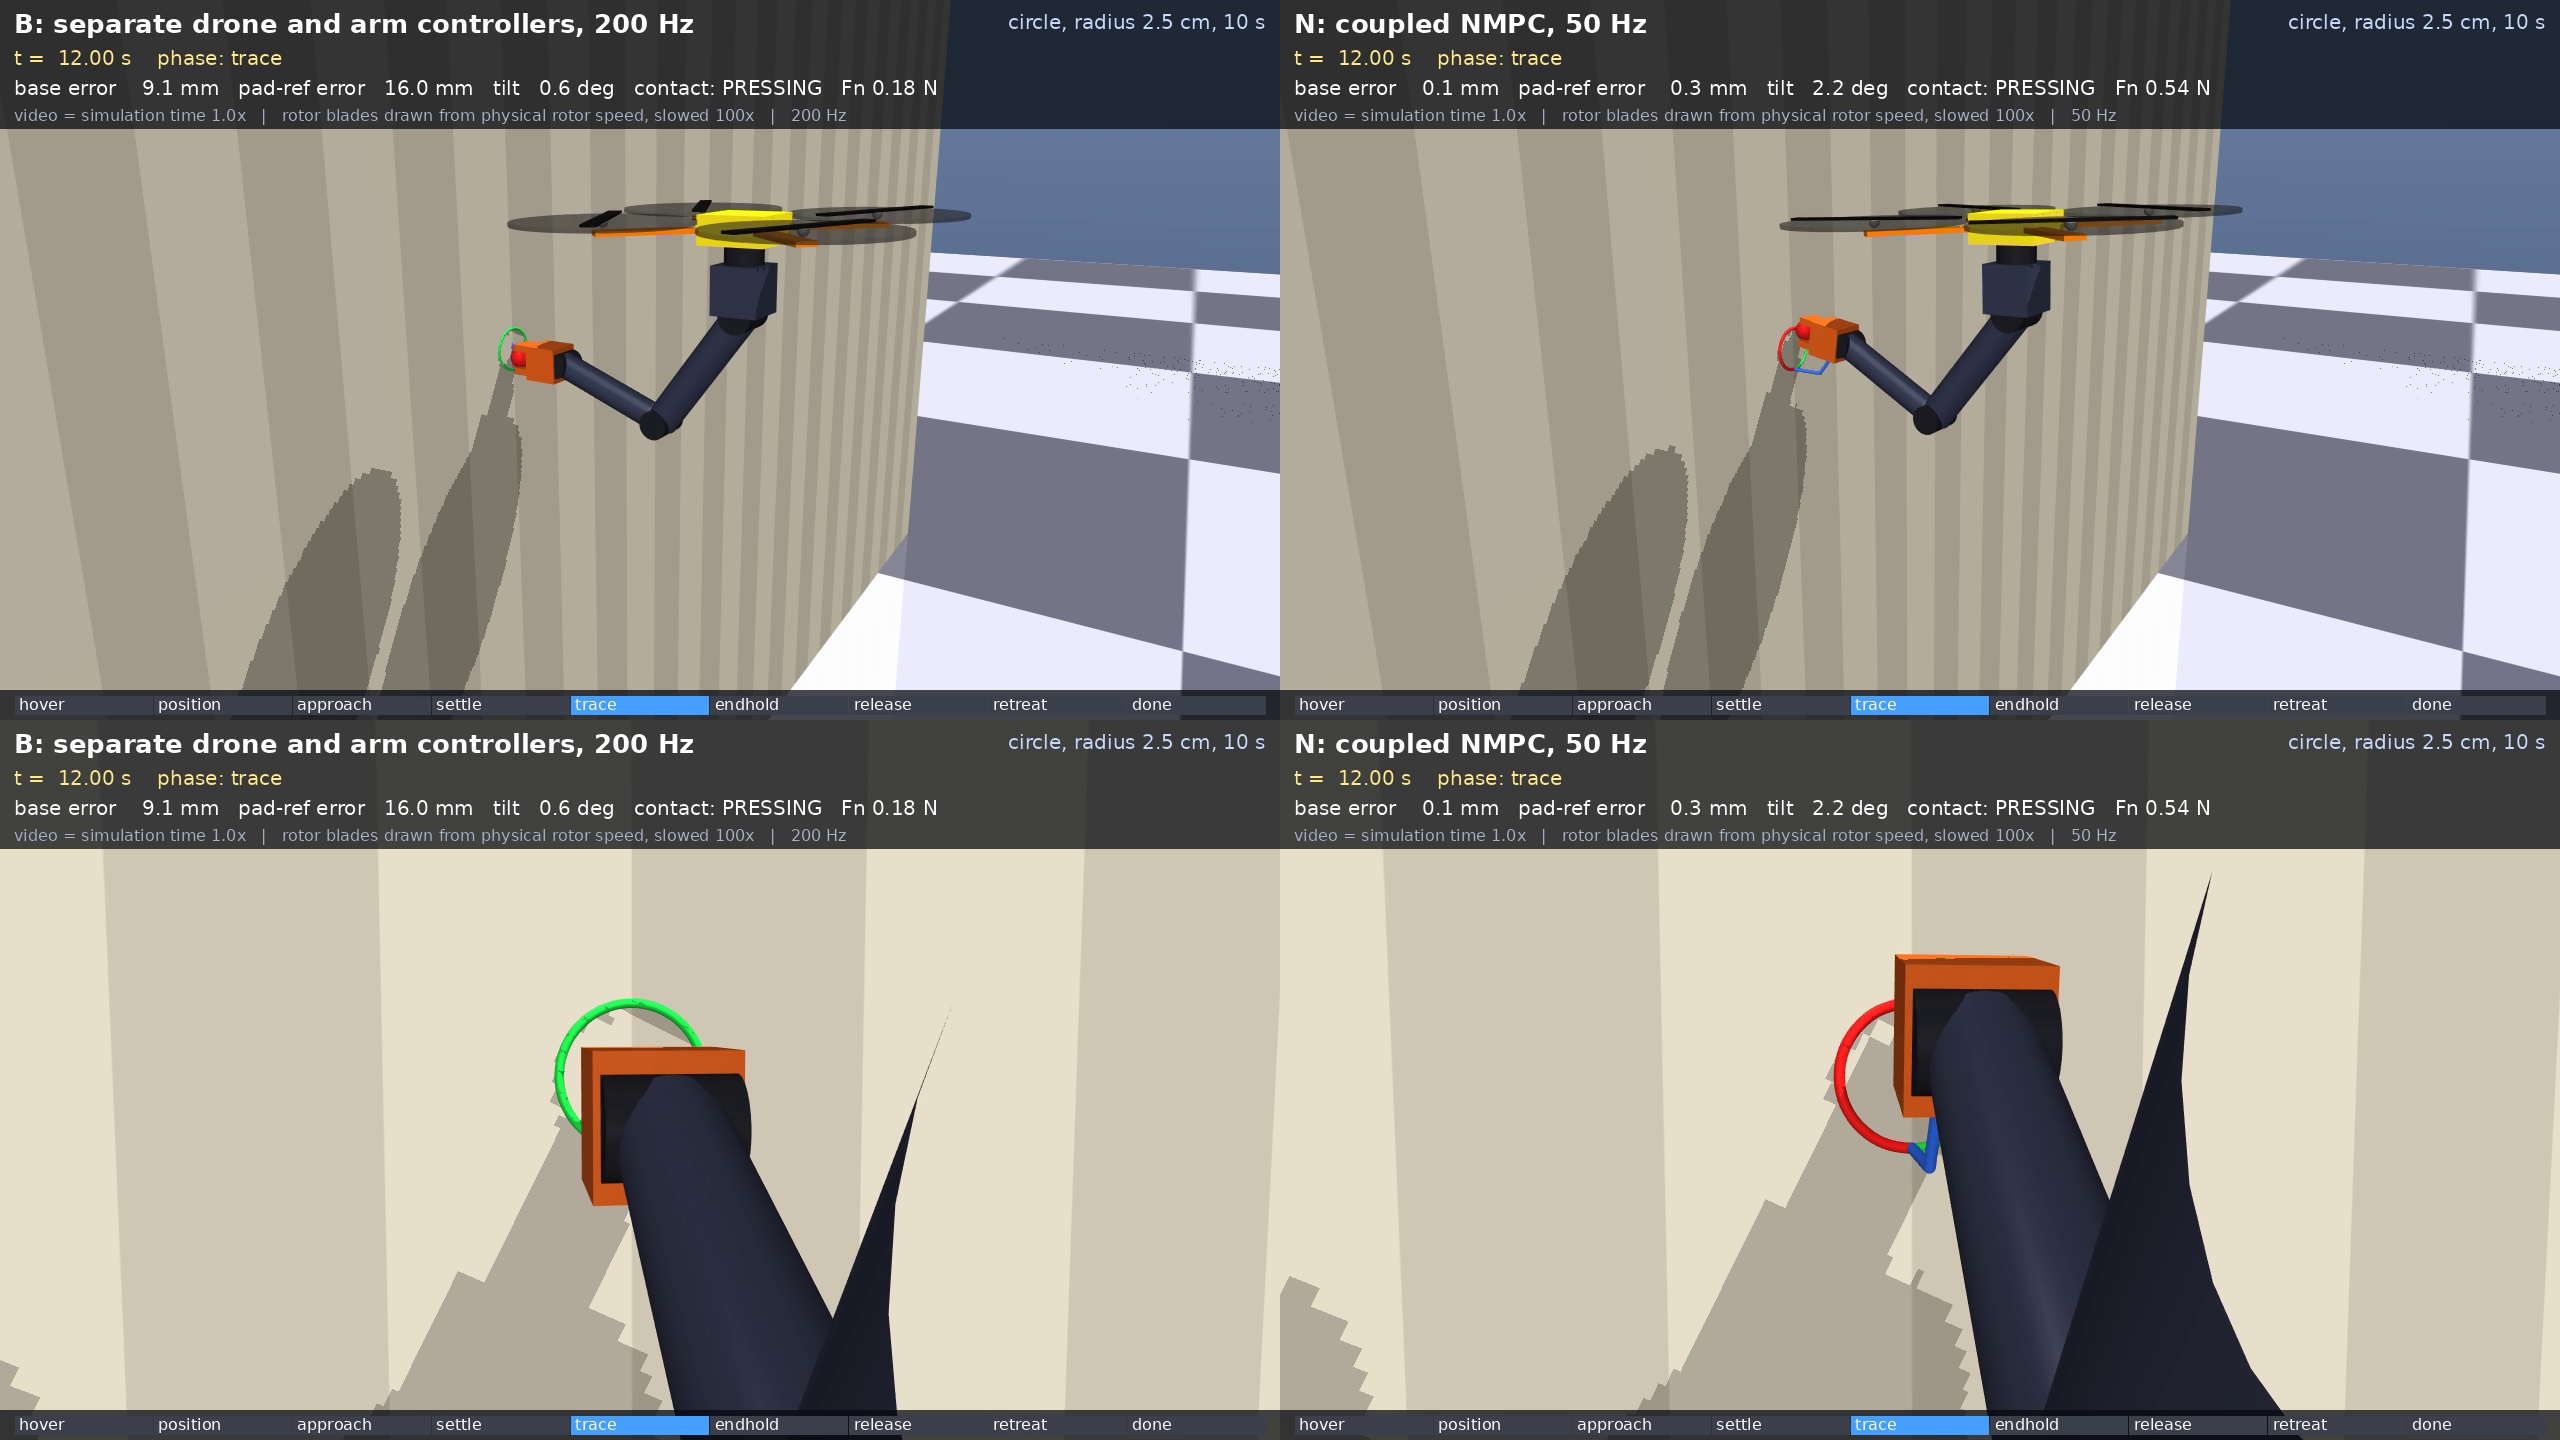
\includegraphics[width=\textwidth]{bn_circle_frame.png}
\caption{Actual B/N simulation frames from the line and circle comparison videos. B is on the left and N on the right; each frame includes overview and wall-facing views. Top: the line at 9.00 s, when B is recovering (15.3 mm base error, 23.4 mm instantaneous pad-reference error) and N is tracing (0.2 mm and 0.5 mm). Bottom: the circle at 12.00 s, with instantaneous pad-reference errors of 16.0 mm for B and 0.3 mm for N. The retained overlays identify controller, time and force. Green is the requested path; the colored traces are visualization overlays, not physical extensions of the arm.}
\label{fig:mediawalls}
\end{figure*}

\begin{figure*}[t]
\centering
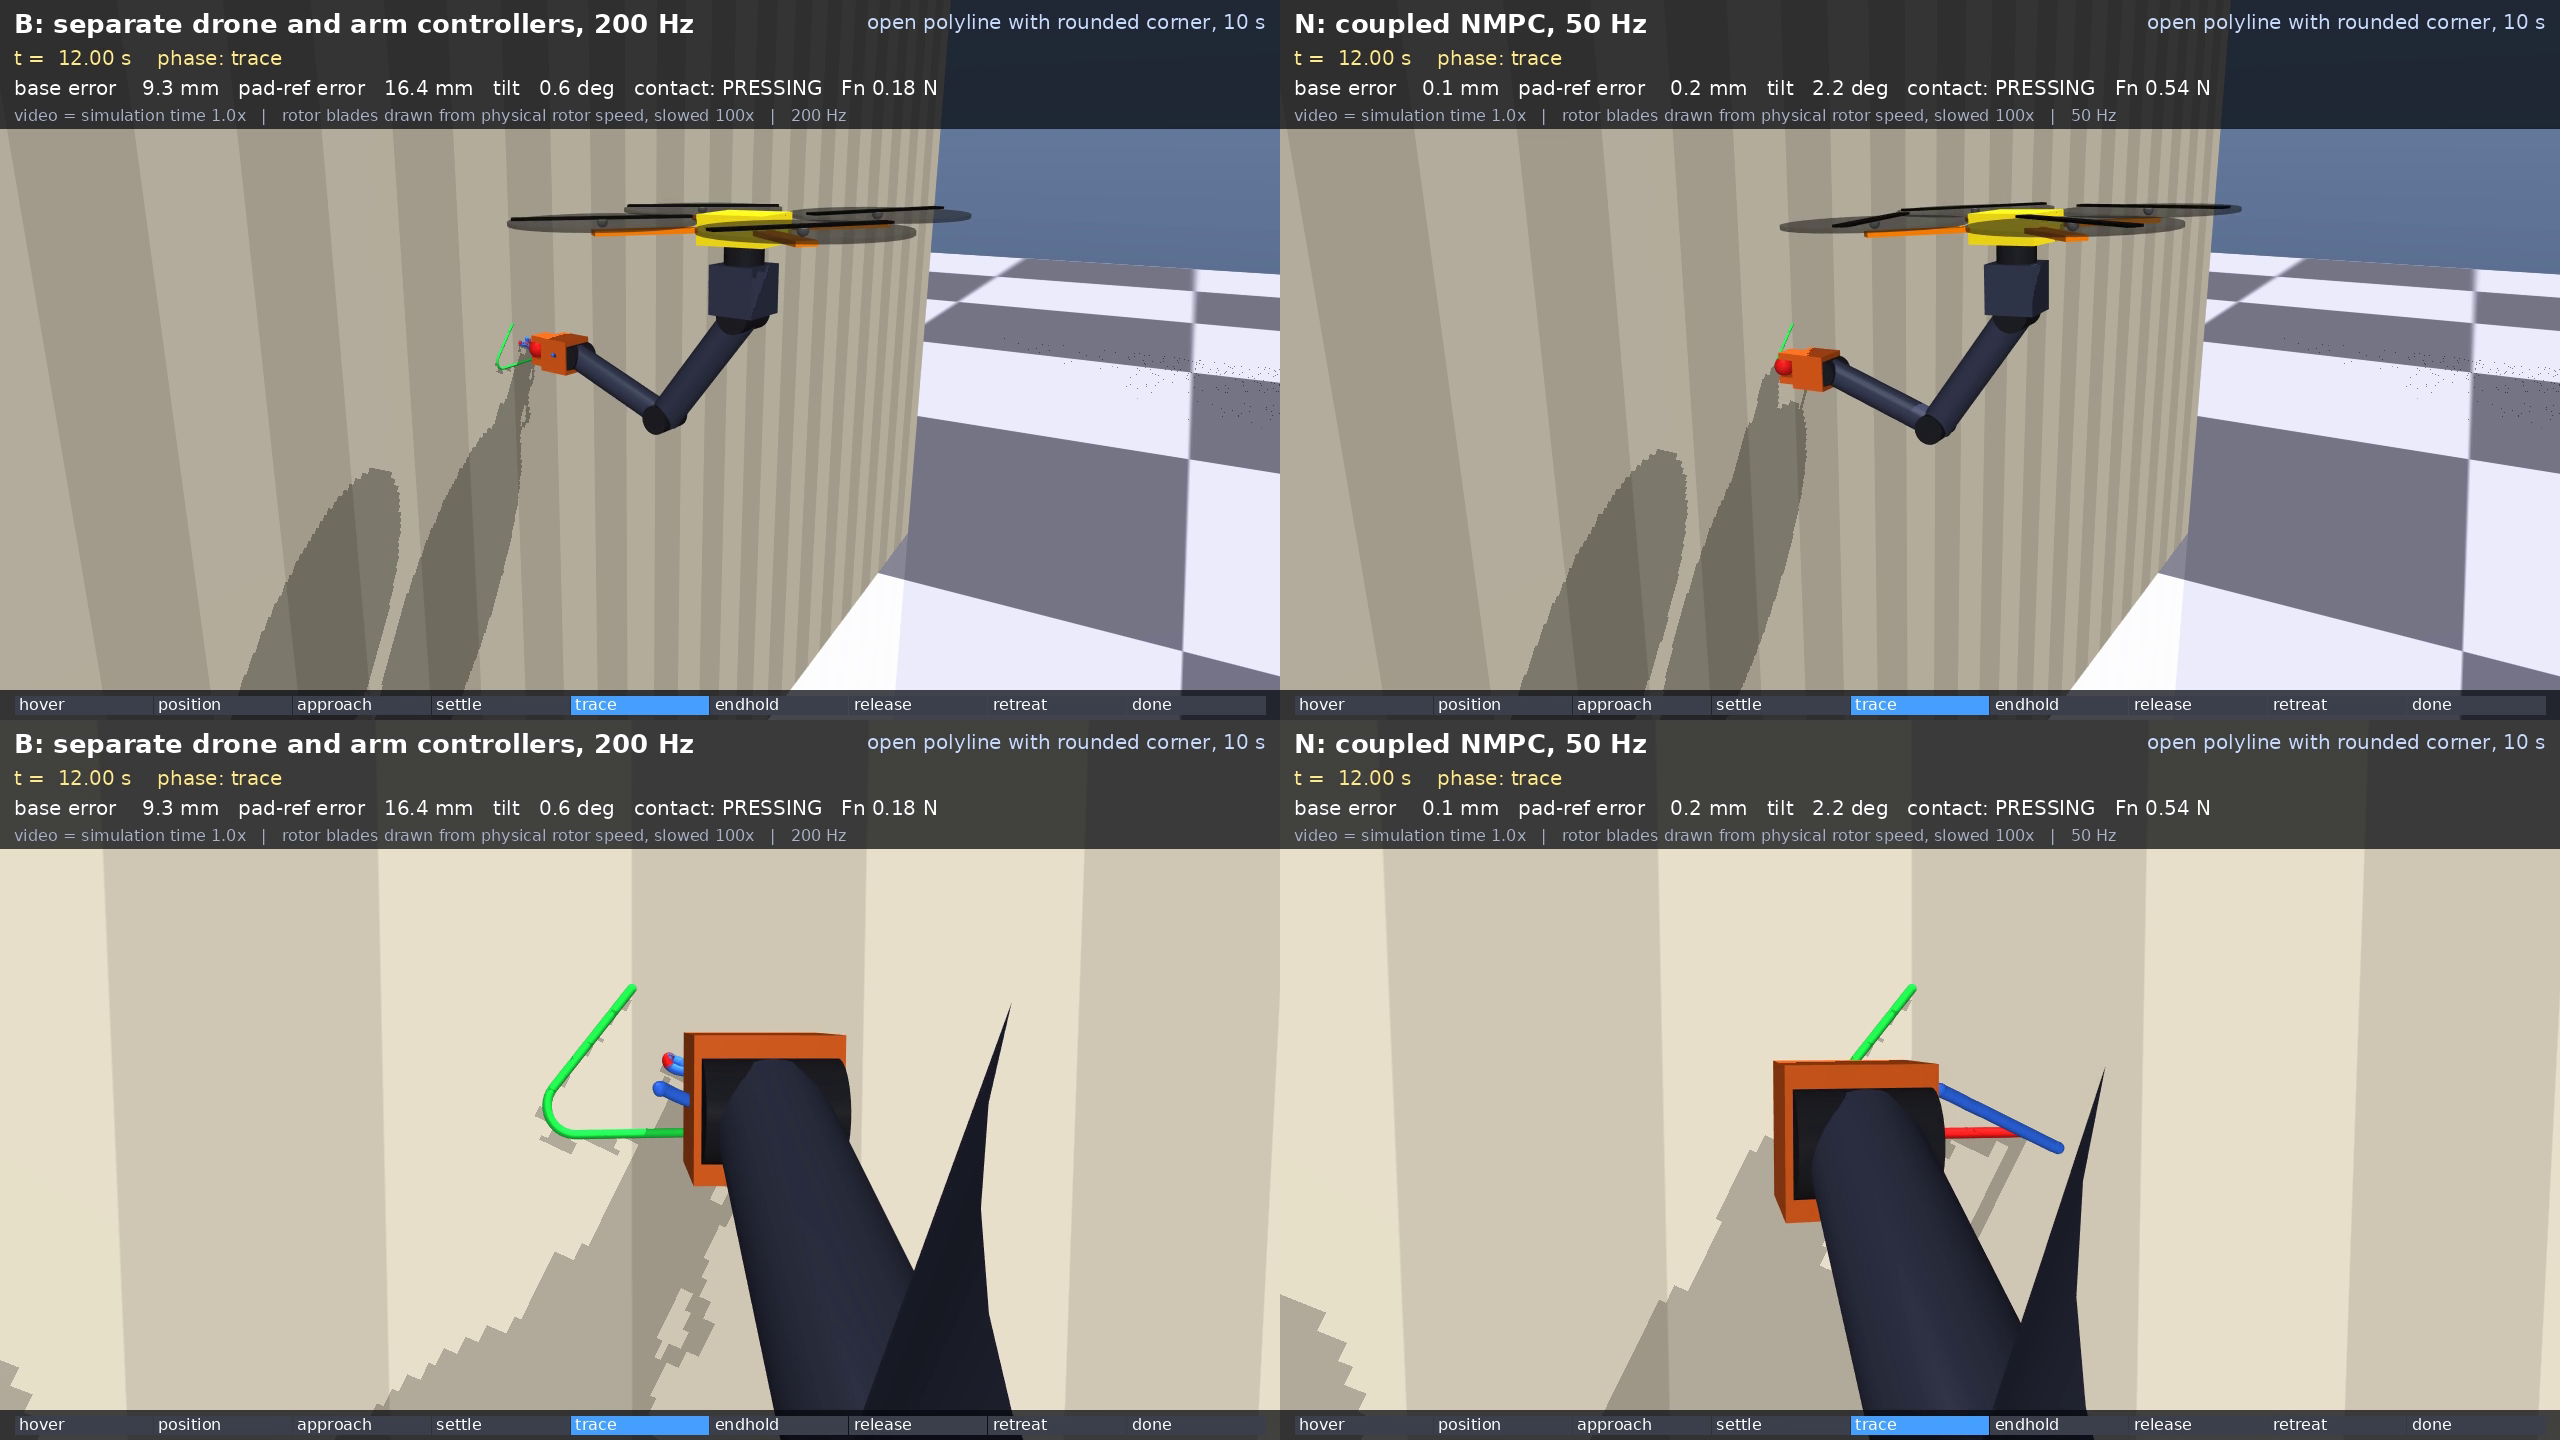
\includegraphics[width=\textwidth]{bn_polyline_frame.png}
\caption{Actual separated-B/N rounded-polyline recording at 12.00 s, B left and N right. The trace is an open polyline with a rounded corner. The snapshot reports base errors of 9.3 mm and 0.1 mm, and instantaneous pad-reference errors of 16.4 mm and 0.2 mm, respectively. The hand contacts the wall directly through its compact pad; displayed paths are graphical traces. This snapshot complements, rather than replaces, whole-run tracking and contact metrics.}
\label{fig:mediapolyline}
\end{figure*}

\begin{figure*}[p]
\centering
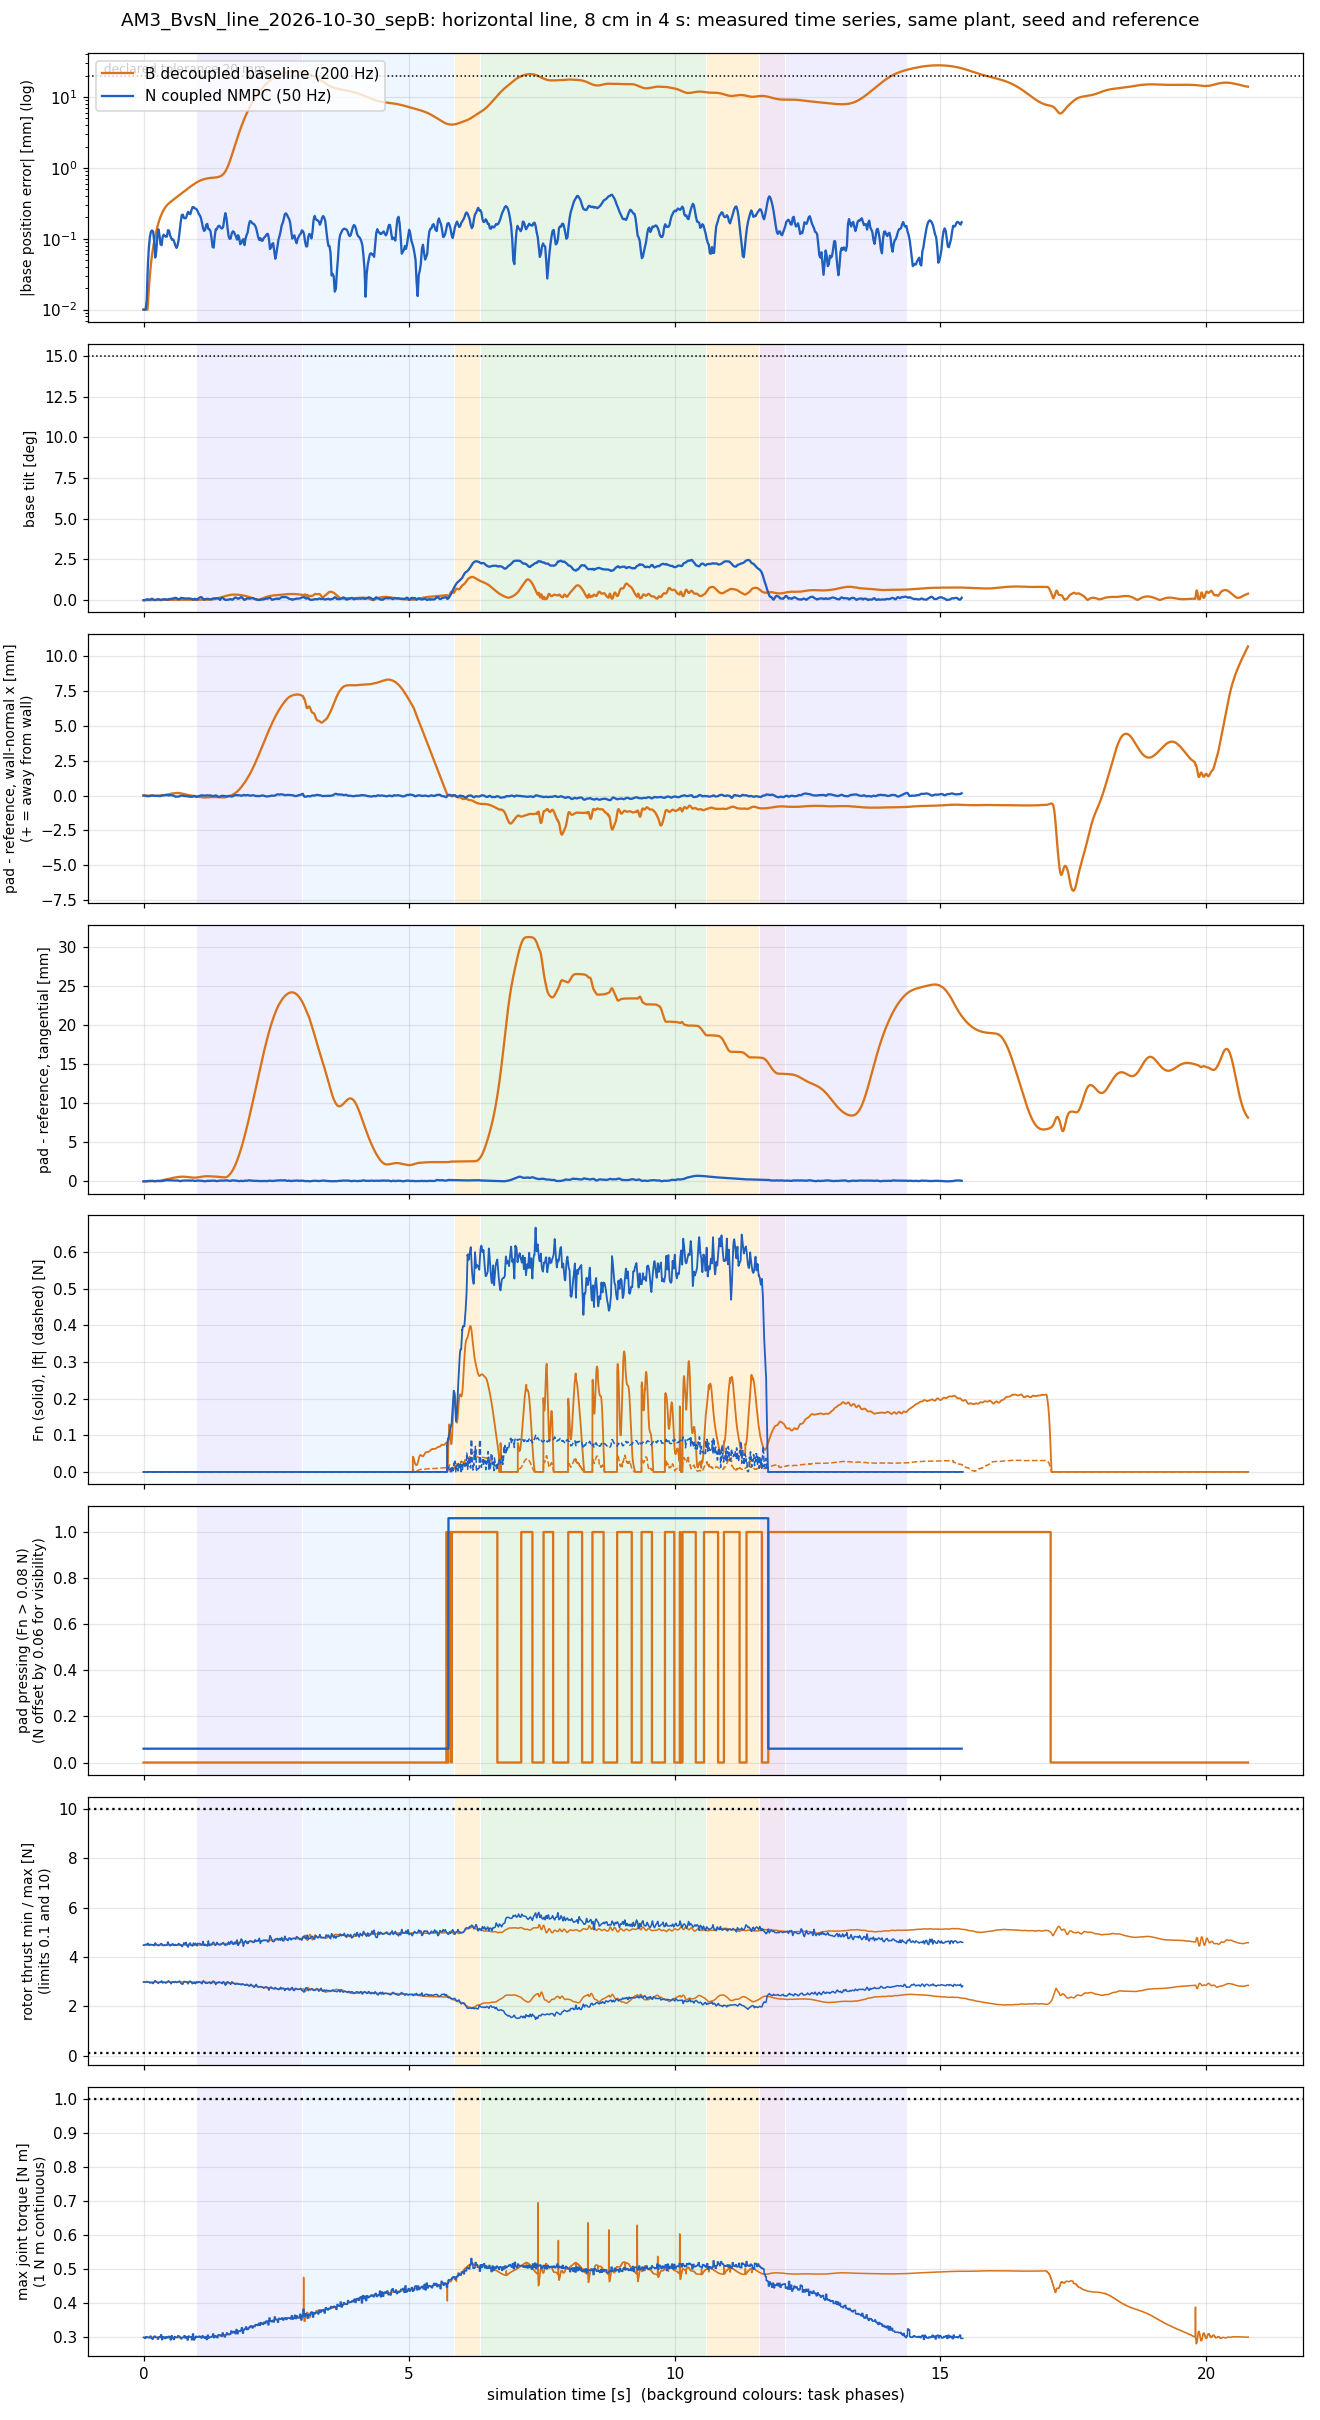
\includegraphics[width=.88\textwidth,height=.85\textheight,keepaspectratio]{bn_line_timeseries.png}
\caption{Eight-panel time series of the B/N horizontal-line recording. Orange denotes B and blue denotes N, consistent with the other report plots. Panels show base error, tilt, wall-normal and tangential pad errors, normal/tangential contact force, pressing status, rotor thrust extrema and maximum joint torque. The base-error axis is logarithmic. The pressing indicator is instantaneous and is distinct from persistence-based contact-loss detection. Background phase colors belong to N; B's recoveries extend its run.}
\label{fig:mediatimeseries}
\end{figure*}

\subsection{Response to arm motion in free flight}
The wall-free test uses the same plant and a task without contact. After 3 s of stationary hover, the pad center follows a circle of radius $A$ in the world $y$--$z$ plane at frequency $f$, with the amplitude ramped in over 1 s. The pad reference is
\begin{equation}
\mathbf p_{T,r}(t)=\mathbf p_{T,0}+r(t)\,A\,(0,\ \sin\omega t,\ 1-\cos\omega t)^T,\quad\omega=2\pi f,
\end{equation}
where $r(t)$ is the fifth-order ramp from 0 to 1 over 1 s. The peak reference speed and acceleration are $A\omega$ and $A\omega^2$; for $A=6$ cm and $f=2$ Hz they are 0.75 m/s and 9.5 m/s$^2$. These are reference quantities, not measured values. Before the motion starts, B holds the base within 0.81 mm and N within 0.16 mm, so any later displacement is caused by the commanded arm motion.

\begin{table*}[t]
\caption{Circle Test Grid, Free Flight, Nominal Plant, Seed 0}
\label{tab:circlegrid}
\centering\footnotesize
\begin{tabular}{cc|cccc|cccc}\hline
 & & \multicolumn{4}{c|}{B} & \multicolumn{4}{c}{N}\\
$A$ (cm) & $f$ (Hz) & Base max & Tilt max & Pad RMS & Abort (s) & Base max & Tilt max & Pad RMS & Abort (s)\\
 & & (mm) & (deg) & (mm) & & (mm) & (deg) & (mm) & \\\hline
2 & 1 & 29.3 & 7.7 & 28.3 & -- & 0.4 & 0.6 & 0.2 & --\\
2 & 1.5 & 13.7 & 3.9 & 11.3 & -- & 0.9 & 1.6 & 0.3 & --\\
2 & 2 & 32.0 & 3.7 & 23.0 & -- & 1.9 & 2.8 & 0.4 & --\\
2 & 3 & 29.7 & 2.6 & 22.6 & -- & 2.2 & 1.9 & 0.6 & --\\
4 & 1 & 68.9 & 16.1 & 61.2 & -- & 0.7 & 1.3 & 0.3 & --\\
4 & 1.5 & 27.0 & 8.4 & 20.4 & -- & 1.8 & 3.2 & 0.5 & --\\
4 & 2 & 39.7 & 4.4 & 29.4 & -- & 3.8 & 5.6 & 0.7 & --\\
4 & 3 & 248.4 & 38.3 & 130.6 & 4.99 & 56.3 & 22.4 & 8.2 & --\\
6 & 1 & 126.7 & 25.4 & 107.7 & -- & 1.0 & 2.2 & 0.5 & --\\
6 & 1.5 & 39.7 & 13.4 & 28.4 & -- & 2.8 & 5.1 & 0.7 & --\\
6 & 2 & 116.2 & 39.9 & 42.9 & 4.85 & 5.9 & 9.9 & 1.2 & --\\
6 & 3 & 225.5 & 39.3 & 65.2 & 4.04 & 102.6 & 38.3 & 25.4 & 6.24\\
\hline
\end{tabular}
\vspace{2pt}

\parbox{.9\textwidth}{\scriptsize Pad RMS is over the 4 s onward window of the motion; B values for aborted runs cover only the time before the abort. Abort is the loss-of-control failsafe (tilt above 40$^\circ$ or base error above 0.25 m), applied identically to both controllers. The grid was fixed before the runs. Wall contact was audited from the logs only for the $A=6$ cm, 2 Hz case below.}
\end{table*}

Table~\ref{tab:circlegrid} shows that B's base displacement grows with amplitude and speed, from 13.7 to 126.7 mm without aborting at the slower settings, while N stays within 6 mm except at the highest speeds. B aborts at 4 cm and 3 Hz, at 6 cm and 2 Hz, and at 6 cm and 3 Hz. N aborts only at 6 cm and 3 Hz, and at 4 cm and 3 Hz it completes with a 56 mm base error and 8.2 mm pad error, which is not a clean success. The clearest separation is therefore the 6 cm, 2 Hz case, where N completes with 5.9 mm maximum base error, 9.9$^\circ$ tilt and 1.2 mm pad RMS error in the motion window.

Figure~\ref{fig:circle} shows this case. B's base error and tilt grow after the motion starts and reach 116 mm and $40^\circ$ at the abort at 4.845 s; the same abort occurs in seeds 1--3 (4.84--4.85 s, base error 114.5--115.7 mm). In the seed-0 logs neither controller has any wall contact (peak normal force 0 N, no unexpected contacts), so the failure is not a collision effect. B's lowest rotor thrust reaches 0.109 N against the 0.1 N limit, so its rotors saturate at the lower limit.

N's completion is not a full acceptance pass. Its minimum downward rotor reserve is 0.021 N and its upward reserve 0.284 N, both below the 0.3 N criterion; its largest rotor-speed change from hover is about 80\%; and the joint rates of the first two joints reach 3.003 rad/s against the 3 rad/s soft limit. The mechanism of B's loss of control is not isolated. Candidate contributors are the arm's changing mass distribution against a fixed hover trim, the arm reaction acting through the base, the fixed-base assumption in the arm's inverse kinematics, and B's 5 ms-versus-20 ms rate and latency difference; none of these was tested separately.

\begin{figure*}[t]
\centering
\begin{minipage}{.49\textwidth}\centering
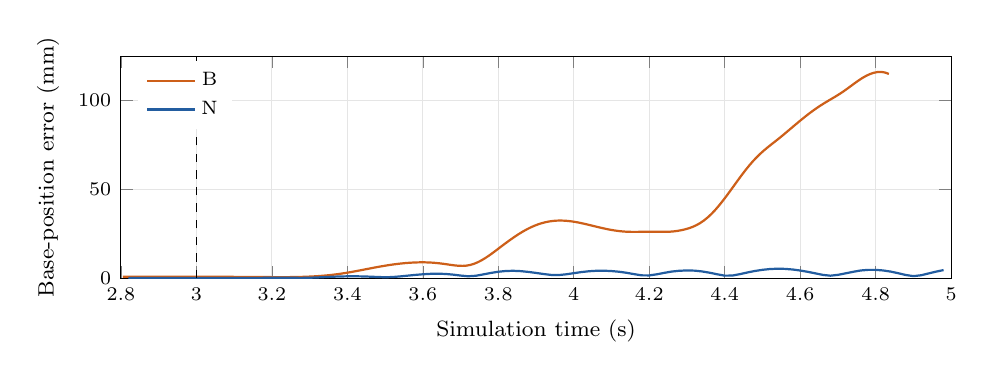
\begin{tikzpicture}
\begin{axis}[width=\linewidth,height=4.4cm,xmin=2.8,xmax=5,ymin=0,ymax=125,xlabel={Simulation time (s)},ylabel={Base-position error (mm)},legend style={at={(.02,.98)},anchor=north west}]
\addplot[baseblue,thick] coordinates {(2.8050,0.8057) (2.8150,0.8067) (2.8250,0.8077) (2.8350,0.8086) (2.8450,0.8096) (2.8550,0.8104) (2.8650,0.8112) (2.8750,0.8117) (2.8850,0.8119) (2.8950,0.8117) (2.9050,0.8112) (2.9150,0.8103) (2.9250,0.8092) (2.9350,0.8079) (2.9450,0.8066) (2.9550,0.8052) (2.9650,0.8037) (2.9750,0.8020) (2.9850,0.8002) (2.9950,0.7981) (3.0050,0.7960) (3.0150,0.7938) (3.0250,0.7914) (3.0350,0.7888) (3.0450,0.7859) (3.0550,0.7827) (3.0650,0.7789) (3.0750,0.7745) (3.0850,0.7694) (3.0950,0.7636) (3.1050,0.7574) (3.1150,0.7503) (3.1250,0.7418) (3.1350,0.7312) (3.1450,0.7177) (3.1550,0.7013) (3.1650,0.6826) (3.1750,0.6628) (3.1850,0.6432) (3.1950,0.6253) (3.2050,0.6106) (3.2150,0.6007) (3.2250,0.5971) (3.2350,0.6012) (3.2450,0.6141) (3.2550,0.6373) (3.2650,0.6723) (3.2750,0.7207) (3.2850,0.7840) (3.2950,0.8638) (3.3050,0.9618) (3.3150,1.0798) (3.3250,1.2199) (3.3350,1.3841) (3.3450,1.5740) (3.3550,1.7911) (3.3650,2.0363) (3.3750,2.3099) (3.3850,2.6114) (3.3950,2.9397) (3.4050,3.2925) (3.4150,3.6670) (3.4250,4.0595) (3.4350,4.4654) (3.4450,4.8793) (3.4550,5.2954) (3.4650,5.7079) (3.4750,6.1112) (3.4850,6.5003) (3.4950,6.8711) (3.5050,7.2197) (3.5150,7.5430) (3.5250,7.8384) (3.5350,8.1036) (3.5450,8.3368) (3.5550,8.5358) (3.5650,8.6986) (3.5750,8.8230) (3.5850,8.9065) (3.5950,8.9459) (3.6050,8.9376) (3.6150,8.8776) (3.6250,8.7621) (3.6350,8.5902) (3.6450,8.3643) (3.6550,8.0920) (3.6650,7.7884) (3.6750,7.4789) (3.6850,7.2008) (3.6950,7.0032) (3.7050,6.9423) (3.7150,7.0740) (3.7250,7.4405) (3.7350,8.0591) (3.7450,8.9218) (3.7550,10.0036) (3.7650,11.2704) (3.7750,12.6851) (3.7850,14.2084) (3.7950,15.7982) (3.8050,17.4100) (3.8150,19.0112) (3.8250,20.5826) (3.8350,22.1091) (3.8450,23.5760) (3.8550,24.9665) (3.8650,26.2636) (3.8750,27.4534) (3.8850,28.5265) (3.8950,29.4760) (3.9050,30.2972) (3.9150,30.9873) (3.9250,31.5446) (3.9350,31.9691) (3.9450,32.2626) (3.9550,32.4293) (3.9650,32.4754) (3.9750,32.4097) (3.9850,32.2421) (3.9950,31.9841) (4.0050,31.6481) (4.0150,31.2471) (4.0250,30.7947) (4.0350,30.3050) (4.0450,29.7926) (4.0550,29.2725) (4.0650,28.7591) (4.0750,28.2644) (4.0850,27.7982) (4.0950,27.3719) (4.1050,26.9967) (4.1150,26.6809) (4.1250,26.4299) (4.1350,26.2484) (4.1450,26.1378) (4.1550,26.0906) (4.1650,26.0907) (4.1750,26.1175) (4.1850,26.1504) (4.1950,26.1732) (4.2050,26.1765) (4.2150,26.1594) (4.2250,26.1313) (4.2350,26.1111) (4.2450,26.1256) (4.2550,26.2051) (4.2650,26.3773) (4.2750,26.6574) (4.2850,27.0393) (4.2950,27.5242) (4.3050,28.1346) (4.3150,28.9041) (4.3250,29.8697) (4.3350,31.0664) (4.3450,32.5194) (4.3550,34.2408) (4.3650,36.2297) (4.3750,38.4724) (4.3850,40.9423) (4.3950,43.6016) (4.4050,46.4032) (4.4150,49.2979) (4.4250,52.2400) (4.4350,55.1815) (4.4450,58.0694) (4.4550,60.8507) (4.4650,63.4807) (4.4750,65.9300) (4.4850,68.1844) (4.4950,70.2487) (4.5050,72.1457) (4.5150,73.9127) (4.5250,75.5965) (4.5350,77.2543) (4.5450,78.9415) (4.5550,80.6856) (4.5650,82.4764) (4.5750,84.2753) (4.5850,86.0642) (4.5950,87.8424) (4.6050,89.6001) (4.6150,91.3106) (4.6250,92.9512) (4.6350,94.5133) (4.6450,95.9983) (4.6550,97.4090) (4.6650,98.7453) (4.6750,100.0178) (4.6850,101.2621) (4.6950,102.5276) (4.7050,103.8577) (4.7150,105.2771) (4.7250,106.7833) (4.7350,108.3450) (4.7450,109.9086) (4.7550,111.4137) (4.7650,112.8003) (4.7750,114.0083) (4.7850,114.9910) (4.7950,115.7098) (4.8050,116.1233) (4.8150,116.1849) (4.8250,115.8451) (4.8350,115.0532)};
\addplot[mpcorange,thick] coordinates {(2.8200,0.1046) (2.8400,0.1107) (2.8600,0.0960) (2.8800,0.0878) (2.9000,0.1031) (2.9200,0.1164) (2.9400,0.1297) (2.9600,0.1404) (2.9800,0.1593) (3.0000,0.1559) (3.0200,0.1408) (3.0400,0.1098) (3.0600,0.0764) (3.0800,0.0615) (3.1000,0.1031) (3.1200,0.1249) (3.1400,0.1382) (3.1600,0.1577) (3.1800,0.2064) (3.2000,0.2683) (3.2200,0.2929) (3.2400,0.2624) (3.2600,0.2082) (3.2800,0.1881) (3.3000,0.2612) (3.3200,0.4149) (3.3400,0.6263) (3.3600,0.8199) (3.3800,0.9679) (3.4000,1.0625) (3.4200,1.0780) (3.4400,1.0114) (3.4600,0.8680) (3.4800,0.6826) (3.5000,0.5477) (3.5200,0.6613) (3.5400,1.0176) (3.5600,1.4452) (3.5800,1.8598) (3.6000,2.2153) (3.6200,2.4578) (3.6400,2.5402) (3.6600,2.3963) (3.6800,2.0259) (3.7000,1.4982) (3.7200,1.0920) (3.7400,1.3665) (3.7600,2.1333) (3.7800,2.9504) (3.8000,3.6325) (3.8200,4.0653) (3.8400,4.1754) (3.8600,3.9748) (3.8800,3.5420) (3.9000,2.9736) (3.9200,2.3585) (3.9400,1.8478) (3.9600,1.7756) (3.9800,2.2035) (4.0000,2.8350) (4.0200,3.4518) (4.0400,3.9205) (4.0600,4.1824) (4.0800,4.2184) (4.1000,4.0319) (4.1200,3.6448) (4.1400,3.0504) (4.1600,2.2883) (4.1800,1.6105) (4.2000,1.5768) (4.2200,2.1921) (4.2400,3.0240) (4.2600,3.7570) (4.2800,4.1954) (4.3000,4.3702) (4.3200,4.2588) (4.3400,3.8183) (4.3600,3.0984) (4.3800,2.2144) (4.4000,1.4451) (4.4200,1.4833) (4.4400,2.2795) (4.4600,3.2207) (4.4800,4.0669) (4.5000,4.7254) (4.5200,5.1690) (4.5400,5.3446) (4.5600,5.2518) (4.5800,4.9063) (4.6000,4.3339) (4.6200,3.5996) (4.6400,2.7463) (4.6600,1.8713) (4.6800,1.4164) (4.7000,1.8974) (4.7200,2.7212) (4.7400,3.5915) (4.7600,4.3393) (4.7800,4.7014) (4.8000,4.6981) (4.8200,4.3612) (4.8400,3.7119) (4.8600,2.8050) (4.8800,1.8083) (4.9000,1.1708) (4.9200,1.6489) (4.9400,2.6765) (4.9600,3.7019) (4.9800,4.5783)};
\addplot[black,dashed,forget plot] coordinates {(3,0)(3,125)};
\legend{B,N}
\end{axis}
\end{tikzpicture}
\end{minipage}\hfill
\begin{minipage}{.49\textwidth}\centering
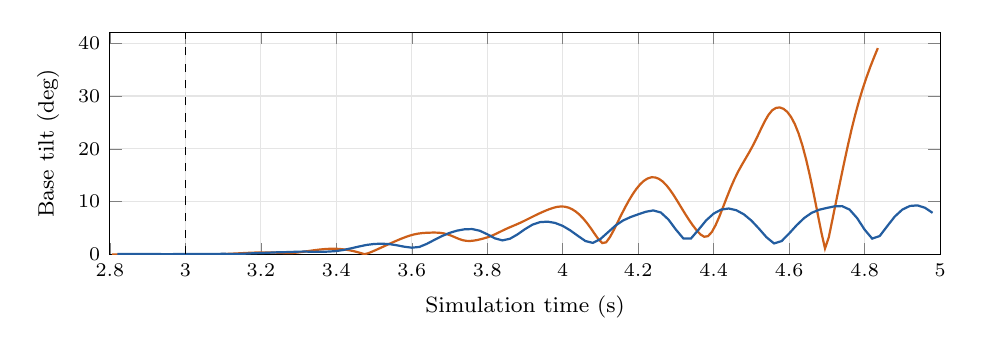
\begin{tikzpicture}
\begin{axis}[width=\linewidth,height=4.4cm,xmin=2.8,xmax=5,ymin=0,ymax=42,xlabel={Simulation time (s)},ylabel={Base tilt (deg)}]
\addplot[baseblue,thick] coordinates {(2.8050,0.0128) (2.8150,0.0121) (2.8250,0.0115) (2.8350,0.0109) (2.8450,0.0105) (2.8550,0.0100) (2.8650,0.0097) (2.8750,0.0096) (2.8850,0.0094) (2.8950,0.0088) (2.9050,0.0081) (2.9150,0.0075) (2.9250,0.0070) (2.9350,0.0067) (2.9450,0.0063) (2.9550,0.0059) (2.9650,0.0055) (2.9750,0.0053) (2.9850,0.0045) (2.9950,0.0030) (3.0050,0.0018) (3.0150,0.0025) (3.0250,0.0044) (3.0350,0.0068) (3.0450,0.0096) (3.0550,0.0132) (3.0650,0.0200) (3.0750,0.0320) (3.0850,0.0496) (3.0950,0.0719) (3.1050,0.0981) (3.1150,0.1275) (3.1250,0.1597) (3.1350,0.1945) (3.1450,0.2315) (3.1550,0.2691) (3.1650,0.3054) (3.1750,0.3376) (3.1850,0.3632) (3.1950,0.3812) (3.2050,0.3908) (3.2150,0.3923) (3.2250,0.3845) (3.2350,0.3672) (3.2450,0.3413) (3.2550,0.3102) (3.2650,0.2819) (3.2750,0.2715) (3.2850,0.2946) (3.2950,0.3541) (3.3050,0.4398) (3.3150,0.5391) (3.3250,0.6427) (3.3350,0.7448) (3.3450,0.8410) (3.3550,0.9277) (3.3650,1.0007) (3.3750,1.0549) (3.3850,1.0856) (3.3950,1.0888) (3.4050,1.0623) (3.4150,1.0047) (3.4250,0.9161) (3.4350,0.7972) (3.4450,0.6484) (3.4550,0.4705) (3.4650,0.2646) (3.4750,0.0581) (3.4850,0.2528) (3.4950,0.5426) (3.5050,0.8536) (3.5150,1.1763) (3.5250,1.5036) (3.5350,1.8303) (3.5450,2.1532) (3.5550,2.4696) (3.5650,2.7765) (3.5750,3.0687) (3.5850,3.3389) (3.5950,3.5786) (3.6050,3.7788) (3.6150,3.9303) (3.6250,4.0303) (3.6350,4.0907) (3.6450,4.1269) (3.6550,4.1458) (3.6650,4.1415) (3.6750,4.0965) (3.6850,3.9900) (3.6950,3.8073) (3.7050,3.5495) (3.7150,3.2437) (3.7250,2.9424) (3.7350,2.7066) (3.7450,2.5787) (3.7550,2.5633) (3.7650,2.6351) (3.7750,2.7646) (3.7850,2.9322) (3.7950,3.1299) (3.8050,3.3630) (3.8150,3.6454) (3.8250,3.9736) (3.8350,4.3264) (3.8450,4.6769) (3.8550,5.0049) (3.8650,5.3099) (3.8750,5.6094) (3.8850,5.9220) (3.8950,6.2567) (3.9050,6.6100) (3.9150,6.9706) (3.9250,7.3267) (3.9350,7.6702) (3.9450,7.9978) (3.9550,8.3072) (3.9650,8.5912) (3.9750,8.8335) (3.9850,9.0085) (3.9950,9.0888) (4.0050,9.0511) (4.0150,8.8790) (4.0250,8.5639) (4.0350,8.1035) (4.0450,7.4996) (4.0550,6.7574) (4.0650,5.8877) (4.0750,4.9103) (4.0850,3.8655) (4.0950,2.8541) (4.1050,2.1618) (4.1150,2.3088) (4.1250,3.2739) (4.1350,4.5957) (4.1450,6.0325) (4.1550,7.4788) (4.1650,8.8747) (4.1750,10.1793) (4.1850,11.3628) (4.1950,12.4006) (4.2050,13.2675) (4.2150,13.9387) (4.2250,14.3927) (4.2350,14.6123) (4.2450,14.5870) (4.2550,14.3155) (4.2650,13.8074) (4.2750,13.0811) (4.2850,12.1670) (4.2950,11.1105) (4.3050,9.9655) (4.3150,8.7879) (4.3250,7.6260) (4.3350,6.5166) (4.3450,5.4851) (4.3550,4.5581) (4.3650,3.7968) (4.3750,3.3549) (4.3850,3.4723) (4.3950,4.2465) (4.4050,5.5392) (4.4150,7.1720) (4.4250,8.9884) (4.4350,10.8472) (4.4450,12.6309) (4.4550,14.2607) (4.4650,15.7088) (4.4750,17.0038) (4.4850,18.2195) (4.4950,19.4468) (4.5050,20.7618) (4.5150,22.1957) (4.5250,23.7045) (4.5350,25.1632) (4.5450,26.4039) (4.5550,27.2818) (4.5650,27.7428) (4.5750,27.8271) (4.5850,27.5751) (4.5950,26.9867) (4.6050,26.0356) (4.6150,24.6858) (4.6250,22.9013) (4.6350,20.6613) (4.6450,17.9743) (4.6550,14.8900) (4.6650,11.4993) (4.6750,7.9233) (4.6850,4.3074) (4.6950,1.1421) (4.7050,3.2498) (4.7150,6.7352) (4.7250,10.2451) (4.7350,13.7233) (4.7450,17.1393) (4.7550,20.4458) (4.7650,23.5618) (4.7750,26.4274) (4.7850,29.0332) (4.7950,31.3932) (4.8050,33.5377) (4.8150,35.5037) (4.8250,37.3296) (4.8350,39.0569)};
\addplot[mpcorange,thick] coordinates {(2.8200,0.0799) (2.8400,0.0975) (2.8600,0.1031) (2.8800,0.1189) (2.9000,0.1148) (2.9200,0.1000) (2.9400,0.0658) (2.9600,0.0698) (2.9800,0.0795) (3.0000,0.0910) (3.0200,0.0940) (3.0400,0.0830) (3.0600,0.0873) (3.0800,0.1055) (3.1000,0.1279) (3.1200,0.1075) (3.1400,0.1025) (3.1600,0.1618) (3.1800,0.2329) (3.2000,0.2768) (3.2200,0.3342) (3.2400,0.4038) (3.2600,0.4377) (3.2800,0.4745) (3.3000,0.5426) (3.3200,0.5504) (3.3400,0.4975) (3.3600,0.5046) (3.3800,0.5520) (3.4000,0.6501) (3.4200,0.8732) (3.4400,1.1802) (3.4600,1.5068) (3.4800,1.8067) (3.5000,1.9895) (3.5200,2.0468) (3.5400,1.9715) (3.5600,1.7486) (3.5800,1.4733) (3.6000,1.2909) (3.6200,1.4284) (3.6400,2.0193) (3.6600,2.7681) (3.6800,3.4848) (3.7000,4.0849) (3.7200,4.5126) (3.7400,4.7703) (3.7600,4.8136) (3.7800,4.4979) (3.8000,3.8337) (3.8200,3.0639) (3.8400,2.6711) (3.8600,2.9739) (3.8800,3.7970) (3.9000,4.7966) (3.9200,5.6528) (3.9400,6.1265) (3.9600,6.2154) (3.9800,5.9689) (4.0000,5.4135) (4.0200,4.5635) (4.0400,3.5398) (4.0600,2.5486) (4.0800,2.1940) (4.1000,2.9306) (4.1200,4.2143) (4.1400,5.4809) (4.1600,6.4384) (4.1800,7.0892) (4.2000,7.6022) (4.2200,8.0874) (4.2400,8.3379) (4.2600,7.9465) (4.2800,6.6293) (4.3000,4.7058) (4.3200,3.0072) (4.3400,3.0404) (4.3600,4.7027) (4.3800,6.4530) (4.4000,7.7451) (4.4200,8.4991) (4.4400,8.7034) (4.4600,8.3762) (4.4800,7.5999) (4.5000,6.4179) (4.5200,4.8917) (4.5400,3.2570) (4.5600,2.0945) (4.5800,2.5365) (4.6000,3.9806) (4.6200,5.5455) (4.6400,6.9114) (4.6600,7.8992) (4.6800,8.4772) (4.7000,8.8119) (4.7200,9.1083) (4.7400,9.1588) (4.7600,8.5028) (4.7800,6.8939) (4.8000,4.7058) (4.8200,3.0045) (4.8400,3.4989) (4.8600,5.3741) (4.8800,7.1901) (4.9000,8.5018) (4.9200,9.1875) (4.9400,9.2936) (4.9600,8.8418) (4.9800,7.8781)};
\addplot[black,dashed,forget plot] coordinates {(3,0)(3,42)};
\end{axis}
\end{tikzpicture}
\end{minipage}
\begin{minipage}{.49\textwidth}\centering
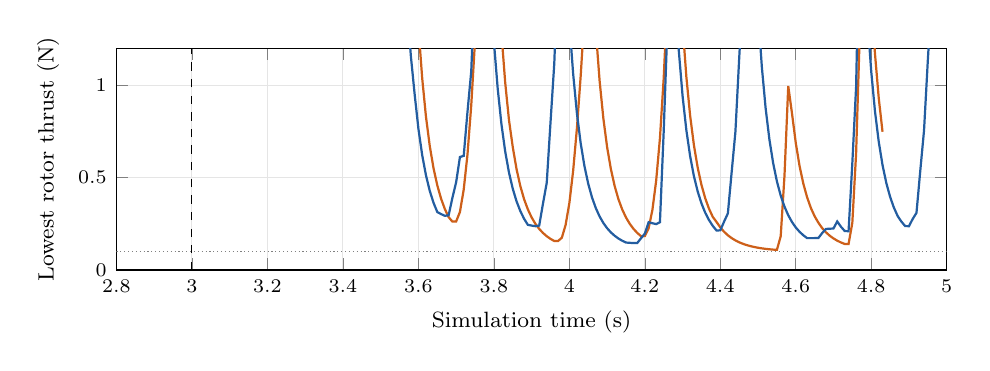
\begin{tikzpicture}
\begin{axis}[width=\linewidth,height=4.4cm,xmin=2.8,xmax=5,ymin=0,ymax=1.2,xlabel={Simulation time (s)},ylabel={Lowest rotor thrust (N)}]
\addplot[baseblue,thick] coordinates {(2.8002,2.9799) (2.8102,2.9785) (2.8202,2.9784) (2.8302,2.9768) (2.8402,2.9768) (2.8502,2.9771) (2.8602,2.9781) (2.8702,2.9794) (2.8802,2.9786) (2.8902,2.9760) (2.9002,2.9747) (2.9102,2.9748) (2.9202,2.9746) (2.9302,2.9746) (2.9402,2.9765) (2.9502,2.9781) (2.9602,2.9792) (2.9702,2.9792) (2.9802,2.9796) (2.9902,2.9784) (3.0002,2.9792) (3.0102,2.9782) (3.0202,2.9777) (3.0302,2.9781) (3.0402,2.9764) (3.0502,2.9717) (3.0602,2.9607) (3.0702,2.9443) (3.0802,2.9245) (3.0902,2.9032) (3.1002,2.8829) (3.1102,2.8657) (3.1202,2.8567) (3.1302,2.8549) (3.1402,2.8559) (3.1502,2.8701) (3.1602,2.8948) (3.1702,2.8853) (3.1802,2.8358) (3.1902,2.7825) (3.2002,2.7299) (3.2102,2.6784) (3.2202,2.6294) (3.2302,2.5848) (3.2402,2.5485) (3.2502,2.5214) (3.2602,2.5089) (3.2702,2.5081) (3.2802,2.5153) (3.2902,2.5420) (3.3002,2.5956) (3.3102,2.6727) (3.3202,2.7732) (3.3302,2.8930) (3.3402,3.0328) (3.3502,3.0069) (3.3602,2.8764) (3.3702,2.7389) (3.3802,2.5982) (3.3902,2.4583) (3.4002,2.3245) (3.4102,2.1961) (3.4202,2.0806) (3.4302,1.9777) (3.4402,1.8905) (3.4502,1.8151) (3.4602,1.7557) (3.4702,1.7138) (3.4802,1.6890) (3.4902,1.6814) (3.5002,1.6816) (3.5102,1.7006) (3.5202,1.7490) (3.5302,1.8301) (3.5402,1.9439) (3.5502,2.0934) (3.5602,2.2762) (3.5702,2.2476) (3.5802,1.9582) (3.5902,1.6481) (3.6002,1.3122) (3.6102,1.0367) (3.6202,0.8289) (3.6302,0.6711) (3.6402,0.5506) (3.6502,0.4578) (3.6602,0.3860) (3.6702,0.3300) (3.6802,0.2860) (3.6902,0.2620) (3.7002,0.2628) (3.7102,0.3141) (3.7202,0.4348) (3.7302,0.6246) (3.7402,0.8914) (3.7502,1.2403) (3.7602,1.6754) (3.7702,2.1942) (3.7802,2.7853) (3.7902,2.7550) (3.8002,2.1128) (3.8102,1.6357) (3.8202,1.2795) (3.8302,1.0121) (3.8402,0.8103) (3.8502,0.6648) (3.8602,0.5457) (3.8702,0.4541) (3.8802,0.3831) (3.8902,0.3278) (3.9002,0.2843) (3.9102,0.2499) (3.9202,0.2225) (3.9302,0.2005) (3.9402,0.1828) (3.9502,0.1685) (3.9602,0.1568) (3.9702,0.1569) (3.9802,0.1745) (3.9902,0.2437) (4.0002,0.3623) (4.0102,0.5364) (4.0202,0.7669) (4.0302,1.0496) (4.0402,1.3836) (4.0502,1.7702) (4.0602,1.6598) (4.0702,1.2976) (4.0802,1.0257) (4.0902,0.8206) (4.1002,0.6648) (4.1102,0.5457) (4.1202,0.4541) (4.1302,0.3831) (4.1402,0.3277) (4.1502,0.2842) (4.1602,0.2498) (4.1702,0.2225) (4.1802,0.2005) (4.1902,0.1828) (4.2002,0.1835) (4.2102,0.2257) (4.2202,0.3248) (4.2302,0.4832) (4.2402,0.7129) (4.2502,1.0385) (4.2602,1.4847) (4.2702,2.0670) (4.2802,2.1901) (4.2902,1.6933) (4.3002,1.3226) (4.3102,1.0445) (4.3202,0.8348) (4.3302,0.6756) (4.3402,0.5540) (4.3502,0.4605) (4.3602,0.3881) (4.3702,0.3316) (4.3802,0.2873) (4.3902,0.2597) (4.4002,0.2303) (4.4102,0.2068) (4.4202,0.1879) (4.4302,0.1726) (4.4402,0.1602) (4.4502,0.1500) (4.4602,0.1417) (4.4702,0.1348) (4.4802,0.1291) (4.4902,0.1244) (4.5002,0.1205) (4.5102,0.1172) (4.5202,0.1145) (4.5302,0.1122) (4.5402,0.1103) (4.5502,0.1094) (4.5602,0.1825) (4.5702,0.5084) (4.5802,0.9951) (4.5902,0.8457) (4.6002,0.6862) (4.6102,0.5621) (4.6202,0.4668) (4.6302,0.3929) (4.6402,0.3354) (4.6502,0.2903) (4.6602,0.2554) (4.6700,0.2269) (4.6800,0.2041) (4.6900,0.1857) (4.7000,0.1709) (4.7100,0.1588) (4.7200,0.1489) (4.7300,0.1407) (4.7400,0.1405) (4.7500,0.2555) (4.7600,0.6302) (4.7700,1.2994) (4.7800,2.2245) (4.7900,1.9167) (4.8000,1.4895) (4.8100,1.1699) (4.8200,0.9296) (4.8300,0.7477)};
\addplot[mpcorange,thick] coordinates {(2.8002,2.9914) (2.8102,2.9335) (2.8202,2.9220) (2.8302,2.9122) (2.8402,2.9139) (2.8502,2.9680) (2.8602,2.9834) (2.8702,2.9973) (2.8802,2.9727) (2.8902,2.9504) (2.9002,2.9506) (2.9102,2.9566) (2.9202,2.9527) (2.9302,2.9282) (2.9402,2.9295) (2.9502,2.9756) (2.9602,2.9871) (2.9702,2.9560) (2.9802,2.9564) (2.9902,2.9697) (3.0002,2.9495) (3.0102,2.9236) (3.0202,2.9240) (3.0302,2.9380) (3.0402,2.9493) (3.0502,2.9685) (3.0602,2.9588) (3.0702,2.9382) (3.0802,2.8742) (3.0902,2.8206) (3.1002,2.8218) (3.1102,2.8655) (3.1202,2.8993) (3.1302,2.9118) (3.1402,2.8908) (3.1502,2.8581) (3.1602,2.8182) (3.1702,2.7847) (3.1802,2.6981) (3.1902,2.6257) (3.2002,2.5974) (3.2102,2.5735) (3.2202,2.5567) (3.2302,2.5426) (3.2402,2.5430) (3.2502,2.5587) (3.2602,2.5714) (3.2702,2.5958) (3.2802,2.6175) (3.2902,2.7236) (3.3002,2.8106) (3.3102,2.9803) (3.3202,3.0277) (3.3302,2.9667) (3.3402,2.7892) (3.3502,2.6432) (3.3602,2.4862) (3.3702,2.3571) (3.3802,2.2381) (3.3902,2.1397) (3.4002,2.0041) (3.4102,1.8927) (3.4202,1.8425) (3.4302,1.8006) (3.4402,1.7694) (3.4502,1.7433) (3.4602,1.7447) (3.4702,1.7944) (3.4802,1.8361) (3.4902,1.9578) (3.5002,2.0577) (3.5102,2.2239) (3.5202,2.3621) (3.5302,2.5217) (3.5402,2.2414) (3.5502,2.0171) (3.5602,1.6842) (3.5702,1.4259) (3.5802,1.1562) (3.5902,0.9500) (3.6002,0.7632) (3.6102,0.6210) (3.6202,0.5121) (3.6302,0.4281) (3.6402,0.3638) (3.6502,0.3135) (3.6602,0.3025) (3.6702,0.2933) (3.6802,0.2958) (3.6902,0.3899) (3.7002,0.4754) (3.7102,0.6112) (3.7202,0.6174) (3.7302,0.8552) (3.7402,1.0756) (3.7502,1.5970) (3.7602,2.0842) (3.7702,2.5540) (3.7802,1.9909) (3.7902,1.5690) (3.8002,1.2347) (3.8102,0.9830) (3.8202,0.7882) (3.8302,0.6401) (3.8402,0.5268) (3.8502,0.4395) (3.8602,0.3717) (3.8702,0.3188) (3.8802,0.2772) (3.8902,0.2443) (3.9002,0.2403) (3.9102,0.2370) (3.9202,0.2400) (3.9302,0.3582) (3.9402,0.4719) (3.9502,0.7975) (3.9602,1.1166) (3.9702,1.6739) (3.9802,2.1148) (3.9902,1.7059) (4.0002,1.3379) (4.0102,1.0612) (4.0202,0.8474) (4.0302,0.6852) (4.0402,0.5614) (4.0502,0.4662) (4.0602,0.3925) (4.0702,0.3351) (4.0802,0.2900) (4.0902,0.2544) (4.1002,0.2261) (4.1102,0.2035) (4.1202,0.1852) (4.1302,0.1704) (4.1402,0.1584) (4.1502,0.1486) (4.1602,0.1471) (4.1702,0.1459) (4.1802,0.1466) (4.1902,0.1721) (4.2002,0.1972) (4.2102,0.2585) (4.2202,0.2530) (4.2302,0.2484) (4.2402,0.2587) (4.2502,0.7522) (4.2602,1.3287) (4.2702,1.8818) (4.2802,1.4843) (4.2902,1.1847) (4.3002,0.9407) (4.3102,0.7561) (4.3202,0.6156) (4.3302,0.5079) (4.3402,0.4249) (4.3502,0.3604) (4.3602,0.3099) (4.3702,0.2702) (4.3802,0.2387) (4.3902,0.2135) (4.4002,0.2148) (4.4102,0.2619) (4.4202,0.3063) (4.4302,0.5283) (4.4402,0.7477) (4.4502,1.1454) (4.4602,1.5158) (4.4702,1.9217) (4.4802,2.1344) (4.4902,1.7900) (4.5002,1.3949) (4.5102,1.0989) (4.5202,0.8759) (4.5302,0.7069) (4.5402,0.5780) (4.5502,0.4790) (4.5602,0.4024) (4.5702,0.3429) (4.5802,0.2961) (4.5902,0.2593) (4.6002,0.2300) (4.6102,0.2066) (4.6202,0.1877) (4.6302,0.1725) (4.6402,0.1725) (4.6502,0.1726) (4.6602,0.1734) (4.6700,0.1997) (4.6800,0.2221) (4.6900,0.2234) (4.7000,0.2244) (4.7100,0.2626) (4.7200,0.2337) (4.7300,0.2106) (4.7400,0.2100) (4.7500,0.5779) (4.7600,0.9907) (4.7700,1.9737) (4.7800,1.6276) (4.7900,1.3617) (4.8000,1.0758) (4.8100,0.8585) (4.8200,0.6936) (4.8300,0.5678) (4.8400,0.4711) (4.8500,0.3964) (4.8600,0.3381) (4.8700,0.2924) (4.8800,0.2619) (4.8900,0.2376) (4.9000,0.2371) (4.9100,0.2764) (4.9200,0.3091) (4.9300,0.5356) (4.9400,0.7549) (4.9500,1.1318) (4.9600,1.4780) (4.9700,1.9380) (4.9800,2.0919) (4.9900,1.7091)};
\addplot[black,dashed,forget plot] coordinates {(3,0)(3,1.2)};
\addplot[gray,densely dotted,forget plot] coordinates {(2.8,0.1)(5,0.1)};
\end{axis}
\end{tikzpicture}
\end{minipage}\hfill
\begin{minipage}{.49\textwidth}\centering
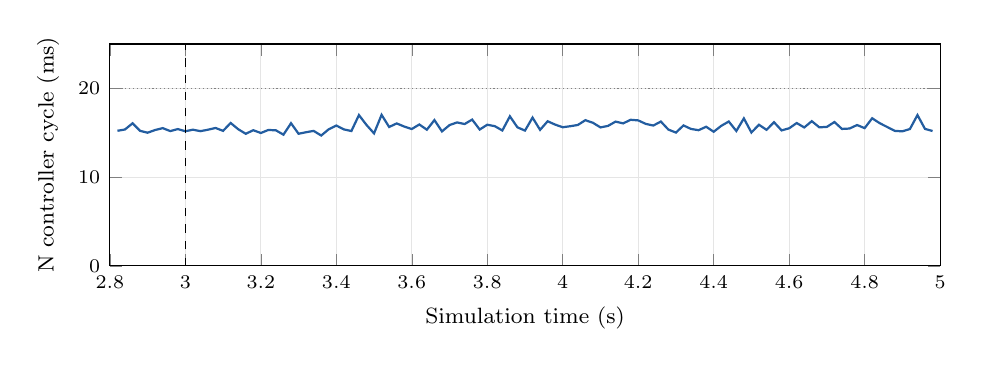
\begin{tikzpicture}
\begin{axis}[width=\linewidth,height=4.4cm,xmin=2.8,xmax=5,ymin=0,ymax=25,xlabel={Simulation time (s)},ylabel={N controller cycle (ms)}]
\addplot[mpcorange,thick] coordinates {(2.8200,15.2165) (2.8400,15.3638) (2.8600,16.0575) (2.8800,15.2138) (2.9000,15.0018) (2.9200,15.3057) (2.9400,15.5176) (2.9600,15.1823) (2.9800,15.4116) (3.0000,15.1660) (3.0200,15.3427) (3.0400,15.1757) (3.0600,15.3393) (3.0800,15.5353) (3.1000,15.2105) (3.1200,16.0981) (3.1400,15.3980) (3.1600,14.8807) (3.1800,15.2799) (3.2000,14.9702) (3.2200,15.3114) (3.2400,15.2682) (3.2600,14.7795) (3.2800,16.0725) (3.3000,14.8818) (3.3200,15.0574) (3.3400,15.2044) (3.3600,14.6828) (3.3800,15.3896) (3.4000,15.8123) (3.4200,15.3749) (3.4400,15.1901) (3.4600,16.9892) (3.4800,15.8741) (3.5000,14.9263) (3.5200,17.0141) (3.5400,15.6465) (3.5600,16.0467) (3.5800,15.6954) (3.6000,15.4162) (3.6200,15.9265) (3.6400,15.3395) (3.6600,16.4223) (3.6800,15.1466) (3.7000,15.8599) (3.7200,16.1596) (3.7400,15.9779) (3.7600,16.4803) (3.7800,15.3582) (3.8000,15.9004) (3.8200,15.7383) (3.8400,15.2536) (3.8600,16.8471) (3.8800,15.6056) (3.9000,15.2395) (3.9200,16.7019) (3.9400,15.3218) (3.9600,16.2911) (3.9800,15.9129) (4.0000,15.6164) (4.0200,15.7336) (4.0400,15.8733) (4.0600,16.4112) (4.0800,16.1194) (4.1000,15.6000) (4.1200,15.7685) (4.1400,16.2512) (4.1600,16.0523) (4.1800,16.4560) (4.2000,16.3883) (4.2200,15.9964) (4.2400,15.8083) (4.2600,16.2585) (4.2800,15.3527) (4.3000,15.0167) (4.3200,15.8207) (4.3400,15.4226) (4.3600,15.2856) (4.3800,15.6720) (4.4000,15.1073) (4.4200,15.7727) (4.4400,16.2635) (4.4600,15.1944) (4.4800,16.6116) (4.5000,15.0241) (4.5200,15.8997) (4.5400,15.3276) (4.5600,16.1799) (4.5800,15.2607) (4.6000,15.4996) (4.6200,16.0906) (4.6400,15.5917) (4.6600,16.3003) (4.6800,15.6048) (4.7000,15.6576) (4.7200,16.2048) (4.7400,15.4263) (4.7600,15.4711) (4.7800,15.8648) (4.8000,15.5160) (4.8200,16.6300) (4.8400,16.0701) (4.8600,15.6429) (4.8800,15.2062) (4.9000,15.1569) (4.9200,15.4165) (4.9400,16.9885) (4.9600,15.4277) (4.9800,15.1953)};
\addplot[black,dashed,forget plot] coordinates {(3,0)(3,25)};
\addplot[gray,densely dotted,forget plot] coordinates {(2.8,20)(5,20)};
\end{axis}
\end{tikzpicture}
\end{minipage}
\caption{Wall-free circle test (6 cm radius, 2 Hz), nominal parameters, seed 0. The dashed vertical line marks the start of the 3 s motion command. B data end at the last logged sample before the abort at 4.845 s; B is not extended or interpolated. Base error and tilt use the logged control samples. Lowest rotor thrust is the 10 ms bin minimum of the four rotor thrusts from the physics-rate samples; the dotted line is the 0.1 N lower thrust limit. N's cycle panel shows the logged cycle times and the 20 ms period.}
\label{fig:circle}
\end{figure*}

\begin{figure*}[t]
\centering
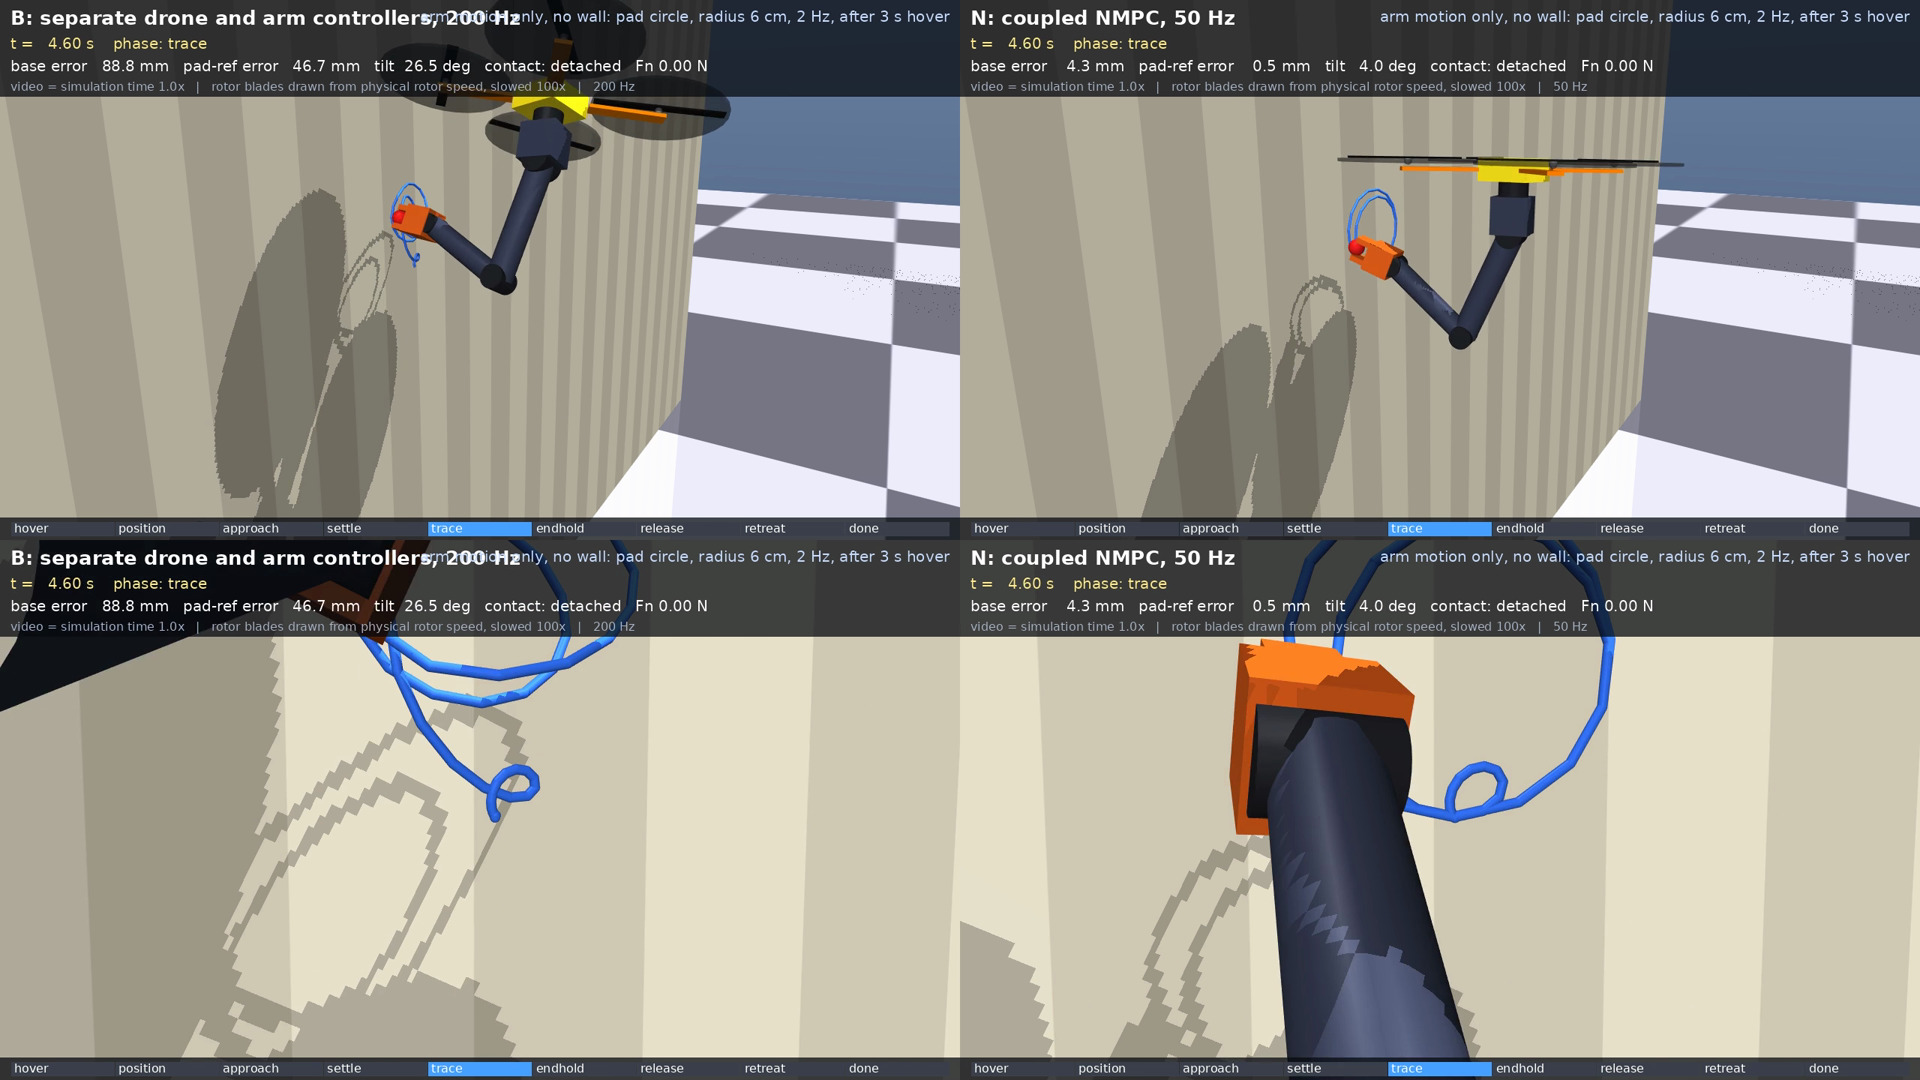
\includegraphics[width=.8\textwidth]{bn_armcircle_frame.png}
\caption{Simulation frame at 4.60 s of the wall-free circle test, overview (top) and wall-facing (bottom) views, B left and N right. B has 88.8 mm base error, 46.7 mm pad-reference error and $26.5^\circ$ tilt; N has 4.3 mm, 0.5 mm and $4.0^\circ$. The overlay text ``no wall'' means that no wall contact is commanded; the wall geometry is present in the plant and the logs record no contact. Blue curves are visualization overlays of the pad path, not physical objects.}
\label{fig:mediacircle}
\end{figure*}

\subsection{Computation and visualization}
In the 6 cm, 2 Hz circle recording, N's full-cycle median is 15.49 ms, the 99th percentile 17.32 ms and the maximum 20.78 ms; 0.36\% of cycles exceed the 20 ms period. Functional simulation uses scheduled command latency, not necessarily actual wall-clock overruns. Neither a median below 20 ms nor a video played at simulation speed establishes real-time operation.

The media consist of frames rendered from live closed-loop simulations, not physical experiments or desktop viewer screen captures. Rotor visualization is slowed for visibility. In the circle comparison, the B panel holds its last frame after the abort with an abort label while N continues; it is not a continued B trajectory. Numerical plots and recorded contact events are necessary to interpret these images.

\section{Current Limitations and Next Steps}
The comparison demonstrates nominal simulation performance. Its interpretation is bounded by the different controller rates and preview horizons, assumed physical parameters, and the use of the nominal plant model within N. The results do not establish hardware performance or isolate the contribution of one coupling term.

The main modeling work remaining is validation of the production prediction step during impact and sliding, inclusion of the joint torque--speed envelope in the predictor, and complete dynamic reachability and collision checks for commanded trajectories. The infeasible reference in the nominal evaluation and the near-zero rotor reserve of N in the circle test make these requirements concrete.

The main implementation requirement is reliable completion of the entire N control cycle within 20 ms. Timing must be assessed with deadline enforcement as well as cycle-time statistics. Further B/N evaluation should use feasible, predeclared tasks and report tracking, contact, actuator margins and timing together. A completed simulation is not a full task pass when one of those criteria is violated.

\section{Conclusion}
A three-joint aerial manipulator has been modeled with a free quadrotor base, articulated arm dynamics, rotor lag and wall contact. B controls the drone and arm independently; N coordinates both through nonlinear predictive control. On the nominal evaluation, N satisfies the functional criteria in 29 of 30 scenarios, compared with 0 of 30 for B. Representative wall trajectories show lower base and end-effector errors and fewer contact losses with N. In a wall-free circle test, B loses control in every tested seed while N completes the motion, although N does so with almost no rotor-thrust reserve. The remaining priorities are dynamic feasibility, prediction accuracy at contact and reliable real-time execution.

\begin{thebibliography}{00}
\bibitem{welde2020} J. Welde and V. Kumar, ``Coordinate-free dynamics and differential flatness of a class of 6DOF aerial manipulators,'' in \textit{Proc. IEEE Int. Conf. Robotics and Automation (ICRA)}, 2020, pp. 4307--4313, doi: 10.1109/ICRA40945.2020.9196705.
\bibitem{welde2021} J. Welde, J. Paulos, and V. Kumar, ``Dynamically feasible task space planning for underactuated aerial manipulators,'' \textit{IEEE Robotics and Automation Letters}, vol. 6, no. 2, pp. 3232--3239, 2021, doi: 10.1109/LRA.2021.3051572.
\bibitem{alharbat2025} A. Alharbat, C. Gabellieri, A. Y. Mersha, and A. Franchi, ``Predictive admittance control for aerial physical interaction,'' \textit{IEEE Robotics and Automation Letters}, accepted-manuscript version, 2025.
\bibitem{mujoco} E. Todorov, T. Erez, and Y. Tassa, ``MuJoCo: A physics engine for model-based control,'' in \textit{Proc. IEEE/RSJ Int. Conf. Intelligent Robots and Systems (IROS)}, 2012, pp. 5026--5033, doi: 10.1109/IROS.2012.6386109.
\bibitem{lynch2017} K. M. Lynch and F. C. Park, \textit{Modern Robotics: Mechanics, Planning, and Control}. Cambridge, U.K.: Cambridge University Press, 2017, chs.~3--5, 8--9, 11--12. doi: 10.1017/9781316661239.
\bibitem{casadi} J. A. E. Andersson, J. Gillis, G. Horn, J. B. Rawlings, and M. Diehl, ``CasADi: A software framework for nonlinear optimization and optimal control,'' \textit{Mathematical Programming Computation}, vol. 11, no. 1, pp. 1--36, 2019, doi: 10.1007/s12532-018-0139-4.
\bibitem{lee2011} T. Lee, M. Leok, and N. H. McClamroch, ``Control of complex maneuvers for a quadrotor UAV using geometric methods on SE(3),'' arXiv:1003.2005, version 4, 2011.
\bibitem{acados} R. Verschueren, G. Frison, D. Kouzoupis, J. Frey, N. van Duijkeren, A. Zanelli, B. Novoselnik, T. Albin, R. Quirynen, and M. Diehl, ``acados: A modular open-source framework for fast embedded optimal control,'' \textit{Mathematical Programming Computation}, vol. 14, no. 1, pp. 147--183, 2022, doi: 10.1007/s12532-021-00208-8.
\bibitem{caccavale2014} F. Caccavale, G. Giglio, G. Muscio, and F. Pierri, ``Adaptive control for UAVs equipped with a robotic arm,'' \textit{IFAC Proceedings Volumes (19th IFAC World Congress, Cape Town)}, vol. 47, no. 3, pp. 11049--11054, 2014.
\bibitem{malczyk2023} G. Malczyk, M. Brunner, E. Cuniato, M. Tognon, and R. Siegwart, ``Multi-directional interaction force control with an aerial manipulator under external disturbances,'' \textit{Autonomous Robots}, vol. 47, pp. 1325--1343, 2023, doi: 10.1007/s10514-023-10128-2.
\bibitem{hui2024} T. Hui, E. Cuniato, M. Pantic, M. Tognon, M. Fumagalli, and R. Siegwart, ``Passive aligning physical interaction of fully-actuated aerial vehicles for pushing tasks,'' in \textit{Proc. IEEE Int. Conf. Robotics and Automation (ICRA)}, 2024, doi: 10.1109/ICRA57147.2024.10610711.
\end{thebibliography}

% Formula-source verification:
% Welde 2020 local Source/icra_2020.pdf: Sec III-B eqs 8, 11-20.
% Caccavale 2014: Source/IFAC14_ifac_final.pdf; Malczyk 2023: Source/s10514-023-10128-2.pdf; Hui 2024: Source/Passive_Aligning_*.pdf; Alharbat 2025: Source/2025-4-RAL.pdf
% https://arxiv.org/pdf/1003.2005 (Lee--Leok--McClamroch v4, Secs II, IV, V)
% https://modernrobotics.northwestern.edu/chapters/chapter8/
% https://modernrobotics.northwestern.edu/nu-gm-book-resource/9-1-and-9-2-point-to-point-trajectories-part-2-of-2/
% https://modernrobotics.northwestern.edu/nu-gm-book-resource/11-4-motion-control-with-torque-or-force-inputs-part-3-of-3/
% https://modernrobotics.northwestern.edu/nu-gm-book-resource/12-2-1-friction/
% Internal experiment provenance (not bibliography entries):
% Plan.md; Code/config/am3_design_v3.json; Code/config/am3_acceptance_v2.json
% Findings/Audits/AM3_B_N_AUDIT_RESPONSE_2026-10-30.md
% Findings/Physics/physics_isolation_2026-10-30.md
% Findings/Codebase/b_separation_2026-10-30.md
% Findings/Codebase/nominal_gate_v2.md
% Findings/Physics/arm_motion_vs_hover_2026-10-30.md
% Publication metadata checked against local Source PDFs and primary sources:
% https://geodesic.mae.cornell.edu/project/aerial-manipulator-flatness
% https://www.kumarrobotics.org/publications/
% https://web.casadi.org/publications/
% https://docs.acados.org/citing/
% https://github.com/google-deepmind/mujoco

% Embedded circle-test plots are derived from:
% Code/results/am3_runs/AM3_BvsN_arm_circle_2Hz_B_loses_control_2026-10-30_{B,N}/log.npz
% Table of the circle grid: Code/results/am3_arm_motion/P_circ/summary.json (seed 0); seeds 1-3: P2_circ/summary.json
% Report preparation source fingerprints (SHA-256, 4 November 2026):
% Code/ocrl/am3_ctrl_b.py
% d931b727aea0c4583a82ba6febbb4d87565dd220e982671afb904692252ab8b4
% Code/ocrl/am3_ctrl_n.py
% 1f8268aea19d86b062355ffc3f6db562a7f53cfa59fdb48e79a0d7484cc34cdc
% Code/ocrl/am3_pred.py
% acf7d9e02aa1ec290d30e7cab58d2dd0f32b40e42a459369723ce33df61f6d6f
% Code/ocrl/am3_nmpc.py
% 4d7e5ef66aa73b67b1468675810062ca0e78bce956d6fd58b28b2be59b583461
% Code/ocrl/am3_plant.py
% 55d02eae2243523bf96c6d13a6ae2e2ab12e375c17fba7c1205c5c0fe2192e05
% Code/ocrl/am3_free_motion.py
% 4481a4a5139060223cfbf3e9b1774e20d0fb1f765214b28945a981d7b4b8763e
% Code/config/am3_design_v3.json
% eb3a0c2edc8bc190209a1302a187d75dedbfa4e5c6e7371e0e2547c8a309b3da
% Code/config/am3_acceptance_v2.json
% 70ac5851e506dd5f43310c22929d9509d8b27adb98d51f22060821c9d9905fc2
% Code/config/am3_task_v1.json
% 45cdf49fc556d4fe7bd88089ebd3c766ddae93b7a9b1a60635173cbb7b29e675
% Code/results/am3_runs/AM3_BvsN_arm_circle_2Hz_B_loses_control_2026-10-30_B/log.npz
% 1fcaa94276517b2ecd49c5c505617a8a646665643a2c60e3fdfedf3761c53f93
% Code/results/am3_runs/AM3_BvsN_arm_circle_2Hz_B_loses_control_2026-10-30_B/summary.json
% ca56793c48742582f793acbdad20de2d75f0753b7302012bf777cebdb97c0007
% Code/results/am3_runs/AM3_BvsN_arm_circle_2Hz_B_loses_control_2026-10-30_N/log.npz
% 937766eb490d2441d6c43a9a834211c65d993b93265803c3fd454d93b2aae4b0
% Code/results/am3_runs/AM3_BvsN_arm_circle_2Hz_B_loses_control_2026-10-30_N/summary.json
% cf3e145d53fb6e46bcd56dd827f08065ea585ea9f284705b1b42672968a562af
% Code/results/am3_arm_motion/P_circ/summary.json
% 9ab2e9c85e01450eba0c7000919c3b65f5bd011732b3ca8eb960de3e8a7ecd71
% Code/results/am3_arm_motion/P2_circ/summary.json
% 43b6d1f00be39873dbdd3d1b9045347766f186908b2a0ab8ef00b52381da1932
% Actual media provenance:
% line: Media_results/AM3_BvsN_line_2026-10-30_sepB/compare_line_overview_wall.mp4, video 9.00 s
% circle (wall): Media_results/AM3_BvsN_circle_2026-10-30_sepB/compare_circle_overview_wall.mp4, video 12.00 s
% polyline: Media_results/AM3_BvsN_rounded_triangle_2026-10-30_sepB/compare_rounded_triangle_overview_wall.mp4, video 12.00 s
% wall-free circle: Media_results/AM3_BvsN_arm_circle_2Hz_B_loses_control_2026-10-30/compare_free_circ_A0.06_f2.0_overview_wall.mp4, frame at 4.60 s
% timeseries: Media_results/AM3_BvsN_line_2026-10-30_sepB/line_timeseries.png (whole figure)
\end{document}
